\documentclass{article}
% Language setting
\usepackage[english]{babel}

% Page geometry
\usepackage[a4paper,top=2cm,bottom=2cm,left=3cm,right=3cm,marginparwidth=1.75cm]{geometry}

% Math and graphics
\usepackage{amsmath, amsfonts}
\usepackage{graphicx}
\usepackage{pgfplots}
\usetikzlibrary{arrows.meta, positioning}
\pgfplotsset{compat=1.18}

% Colors and hyperlinks
\usepackage[dvipsnames]{xcolor}
\usepackage[colorlinks=true, allcolors=blue]{hyperref}

% Listings setup (solo listings, niente minted)
\usepackage{listings}

% --- Color palette (coerente e leggibile) ---
\definecolor{codebg}{RGB}{250,250,250}
\definecolor{coderule}{RGB}{220,220,220}
\definecolor{codekw}{RGB}{0,102,204}
\definecolor{codecomment}{RGB}{90,90,90}
\definecolor{codestring}{RGB}{163,21,21}
\definecolor{codenumber}{RGB}{130,130,130}

% --- Stile per C++ ---
\lstdefinestyle{cppstyle}{
	language=C++,
	backgroundcolor=\color{codebg},
	basicstyle=\linespread{1.1}\ttfamily\small,
	keywordstyle=\color{codekw}\bfseries,
	commentstyle=\color{codecomment}\itshape,
	stringstyle=\color{codestring},
	numbers=left,
	numberstyle=\tiny\color{codenumber},
	numbersep=8pt,
	frame=tb,
	rulecolor=\color{coderule},
	showstringspaces=false,
	breaklines=true,
	tabsize=4,
	captionpos=b,
	aboveskip=1em, belowskip=1em,
	morekeywords={
		std,vector,array,unique_ptr,shared_ptr,nullptr,override,constexpr,decltype,
		uint64_t,int32_t,int64_t,size_t
	}
}

\lstset{style=cppstyle}
\title{Numerical Methods for Soft Matter: Exercises}
\author{Lorenzo Rizzi}
\date{}

\begin{document}
	\maketitle
	
	
	\section{Exercise 1}
	
	\subsection{Inversion method}
	Use the inversion method to design an algorithm that samples random numbers according to the PDF:
	\begin{equation}
		f(x) = (1-x)a+xb \quad\quad\mbox{         with          } x \in [0,1]
		\label{eq::bilinear}
	\end{equation}
	with $a, b \geq 0$. Simulate the designed algorithm with $a = 0$ and $b = 7$ and compare the obtained histograms
	with the analytical expressions
	\textbf{\\ Resolution \\}
	We will use the inversion method to sample from the target distribution $f(x)$. But first of all, we need to normalize it:
	$$
	C = \int_0^1 f(x)dx = \int_0^1 [(1-x)a+xb] dx  = \int_0^1 (x(b-a)+a)dx = \frac{1}{2}(b-a)+a = \frac{1}{2}(b+a)
	$$
	Finally, the normalized distribution looks like:
	$$
	\rho(x) = \frac{f(x)}{C} = \frac{2(1-x)a+2bx}{b+a}
	$$
	Now we can compute the cumulative distribution function $F(x)$:
	$$
	F(x) = \frac{1}{C} \int_0^x ds (s(b-a)+a) = \frac{2}{a+b}\Bigl(\frac{1}{2}(b-a)x^2+ax\Bigl) = \frac{b-a}{b+a}x^2 + \frac{2a}{a+b}x
	$$
	which is injective in $[0,1]$, as desired from a CDF. To invert it, let $F(x)=y$:
	$$
	(a+b)y = (b-a) x^2 + 2a x
	$$
	$$
	x^2 + \frac{2a}{b-a} x - \frac{b+a}{b-a} y = 0
	$$
	and:
	$$
	x = \frac{-\frac{2a}{b-a}\pm \sqrt{\frac{4a^2}{(b-a)^2}-4\frac{b+a}{b-a}}}{2} = \frac{-\frac{2a}{b-a}\pm \sqrt{\frac{4a^2}{(b-a)^2}-4\frac{b+a}{(b-a}}}{2}
	$$
	simplifying further, we finally get:
	$$
	F^{-1}(x) = \frac{\sqrt{a^2 (1-x) + b^2 x}-a}{b-a}
	$$
	To sample from $\rho(x)$, one just has to extract a random real number $\xi_i\in[0,1]$ uniformly and perform:
	$$
	a_i = F^{-1}(\xi_i)
	$$
	and $a_i$ will be distributed according to $\rho$. A snippet of the function used to sample from the target distribution is shown in the following:
	\begin{lstlisting}
		def sampleCustom(n,a,b):
		#First of all, draw n uniform random number between 0 and 1
		u = np.random.uniform(0,1,n)
		#Then, use the inverse CDF to transform the uniform random number 
		z = (np.sqrt(a**2 * (1-u) + b**2 * u) - a) / (b - a)
		return z
	\end{lstlisting}
	The generation of the uniformly distributed numbers is obtained through Numpy's function \texttt{np.random.uniform} that should use MT19937 (Mersenne twister algorithm) under the hood. To verify whether our function properly generate numbers distributed according to $\rho$, we can build a histogram starting from the simulated data and confront it with the actual PDF (Fig.\ref{fig:ex1.1})   
	
	\begin{figure}
		\centering
		\includegraphics[scale=0.6]{./fig/exercise1_1.pdf}
		\caption{\textit{Empirical samples obtained through the inversion method. Here, we generated $n = 100000$ samples with parameters $a = 0, b = 7$. The black solid line represents the theoretical pdf, which nicely fit the generated dataset}}
		\label{fig:ex1.1}
	\end{figure}
	
	\subsection{Estimating areas by MC}
	\paragraph{Part 1}
	Generate random points uniformly distributed within an ellipse of major and minor axes, respectively $a = 5$ and $b = 1$, and compare the analytic value of its area with the Monte Carlo estimate based on the hit-miss method as a function of the number of “throws”
	\textbf{\\Resolution\\}
	We will use the \textit{hit and miss algorithm}. We will generate pairs of points $(x,y)$ uniformly distributed in the rectangle $[-5,5]\times[-1,1]$, i.e. $x\sim\mathcal{U}[-5,5]$, $y\sim\mathcal{U}[-1,1]$. If $\frac{x^2}{a^2}+\frac{x^2}{b^2} \geq 1$, we discard the pair $(x,y)$, otherwise we'll keep it. Results are shown in Fig.\ref{fig:ex12}
	
	To estimate the area of the ellipse, we just have to count the number of "hits". The estimate will then be:
	$$
	A_n = 4\frac{\#\mbox{points in}}{n} ab
	$$
	whereas the actual value of $A$ is $A = \pi a b$. In Fig.\ref{fig:ex12}, right panel, we compare the analytic value of the area $A$ with the Monte Carlo estimate based on
	the hit-miss method as a function of the number of “throws" ($n$), $A_n$. For each value of $n$, we repeat the hit and miss procedure $k=10$ times and average over the results to get a more robust scaling law. The absolute error is obtained as $\epsilon_n = |A-A_n|$, where $A_n$ is the average over the $k = 10$ repetitions. As expected, the scaling behaviour closely resembles the correct one, i.e.:
	$$
	\epsilon_n \sim \frac{1}{\sqrt{n}}
	$$
	This is due to the central limit theorem.
	\begin{figure}[]
		\centering
		\raisebox{-35pt}[\dimexpr\height][\depth]{%
			\includegraphics[width=0.49\linewidth]{./fig/exercise1_2.pdf}%
		}
		\hfill
		\raisebox{0pt}[\dimexpr\height][\depth]{%
			\includegraphics[width=0.49\linewidth]{./fig/exercise1_3.pdf}%
		}
		\caption{\textit{On the left, random points uniformly distributed in an ellipse, using hit and miss method. On the right, scaling law on the absolute error between $A_n$ and $A$, with $n$ ranging from $10^0$ to $10^{7.5}$. The dotted line represents a $O(n^{-1/2})$ scaling behaviour.}}
		\label{fig:ex12}
	\end{figure}
	\paragraph{Part 2}
	Use the hit-and-miss method to generate points within the region $\Omega$ coming from the intersection of the two parabolas $y = x^2$ and $y = 4x - x^2$ and compare the estimate of the area with the analytical expression, again as a function of the number of “throws”
	\textbf{\\Resolution\\}
	The procedure is basically the same as the one in Part 1. The results are shown in Fig.\ref{fig:ex122}.
	\begin{figure}[]
		\centering
		\raisebox{-35pt}[\dimexpr\height][\depth]{%
			\includegraphics[width=0.49\linewidth]{./fig/exercise1_3_points.pdf}%
		}
		\hfill
		\raisebox{0pt}[\dimexpr\height][\depth]{%
			\includegraphics[width=0.49\linewidth]{./fig/exercise1_3_omega.pdf}%
		}
		\vspace{20pt}
		\caption{\textit{On the left, random points uniformly distributed in the plane region between the curve $y = x^2$ and $y = 4x - x^2$, using hit and miss method. On the right, scaling law on the absolute error between $A_n$ and $A$, with $n$ ranging from $10^0$ to $10^{7.5}$. The dotted line represents a $O(n^{-1/2})$ scaling behaviour.}}
		\label{fig:ex122}
	\end{figure}
	\subsection{Sampling by transformation of coordinates}
	The bilinear function
	$$
	f(x, y) = a_0 (1 - x)(1 - y) + a_1 x(1 - y) + a_2 y(1 - x) + a_3 xy
	$$
	interpolates between four values $w_i$ at the four corners of the unitary square $[0, 1]^2$. Normalize the function to get the corresponding PDF $\rho(x, y)$; Write an algorithm that samples random points $(x,y)$ distributed according to $\rho(x, y)$
	\textbf{\\Resolution\\}
	Let's first normalize the PDF:
	$$
	C = \int_0^1\int_0^1 dx dy f(x,y) = \int_0^1\int_0^1 dx dy [a_0 (1 - x)(1 - y) + a_1 x(1 - y) + a_2 y(1 - x) + a_3 xy] = \frac{1}{4}(a_0+a_1+a_2+a_3)
	$$
	If the PDF were separable, then we could have just sampled from the two factorized 1-point PDFs. Unfortunately, this is not the case.
	To sample a pair $(x,y)$ from the target distribution $\rho = \frac{f(x,y)}{C}$, we must first build the marginal distribution on $X$:
	\begin{equation}
		\begin{split}
			p_X(x) &= \frac{1}{C}\int_0^1 dy [a_0 (1 - x)(1 - y) + a_1 x(1 - y) + a_2 y(1 - x) + a_3 xy] \\
			&= \frac{1}{2C}[(a_0+a_2)(1-x)+(a_1+a_3)x] = \frac{2(a_0+a_2)(1-x)+2(a_1+a_3)x}{a_0+a_1+a_2+a_3} 
		\end{split}
	\end{equation}
	Note that this equation is fundamentally the same as the one in Eq.\ref{eq::bilinear}:
	\begin{equation}
		p_X(x) = \frac{2(a_0+a_2)}{a_0+a_1+a_2+a_3}(1-x) + \frac{2(a_1+a_3)}{a_0+a_1+a_2+a_3}x
	\end{equation}
	so we can reuse the same algorithm as the one implemented in exercise 1 with $a = 2(a_0+a_2)$, $b = 2(a_1+a_3)$
	Now we need to sample $y$ from $P(y|x)$, which is given by:
	$$
	p(y|x) = \frac{\rho_{X,Y}(x,y)}{p_X(x)} = \frac{2a_0(1-x)(1-y)+2a_1(1-y)x+2a_2y(1-x)+2a_3xy}{(a_0+a_2)(1-x)+(a_1+a_3)x}
	$$
	which can be rewritten as:
	$$
	p(y|x) = (1-y)\frac{2a_0(1-x)+2a_1x}{(a_0+a_2)(1-x)+(a_1+a_3)x} +y \frac{2a_2(1-x)+2a_3x}{(a_0+a_2)(1-x)+(a_1+a_3)x}
	$$
	which, again, has the same form as in Eq.\ref{eq::bilinear} with $a = 2a_0(1-x)+2a_1x$ and $b = 2a_2(1-x)+2a_3x$. Using the previous algorithm for both $x$ and $y$, we can finally sample a pair $(x,y)$ according to $\rho(x,y)$. Results are shown in Fig.\ref{fig:ex2} with $n = 100000, a_0 = 10,a_1=8, a_2 =2, a_3=0$
	\begin{figure}
		\centering
		\includegraphics[scale=0.425]{./fig/3D_histogram_vs_surface.pdf}
		\caption{\textit{Empirical samples obtained with the marginal and conditional distributions, using inverse method for 1D PDF sampling. We first sample $x$ from its own marginal distribution (a bilinear function) and then we sample $y$ conditioned on $x$ (again, a bilinear function)}}
		\label{fig:ex2}
	\end{figure}
	
	\subsection{Rejection method}
	Using a pseudo-random generator that samples numbers according to the normal distribution, apply the rejection method to generate pseudo-random numbers with the distribution
	\begin{equation}
		\rho(x) = \frac{e^{- x^2/2}}{M (1 + x^2)}
		\label{eq:pdf}
	\end{equation}
	where $M$ is the normalization constant
	\textbf{\\Resolution\\}
	We can't just use the inverse method here because the inverse cumulative distribution $F^{-1}(x)$ has no analytical form. In fact, the normalization constant $M$:
	$$
	M = \int dx \frac{e^{- x^2/2}}{1 + x^2}
	$$
	can't be solved as a function of standard analytical functions\footnote{One could rewrite $M$ in terms of the error function, but we'd still have the problem of inverting a function that is both exponential and quadratic in $x$.}. Therefore, we have to rely on Von Neumann's rejection method. In order to implement this algorithm, we first have to build a PDF $g(x)$ according to two criterions:
	\begin{itemize}
		\item Sampling from $g$ should be easy and straightforward
		\item Given a $c \in \mathbb{R}$, we must have $\rho(x) \leq c g(x), \forall x \in \mathbb{R}$.
	\end{itemize} 
	Let's choose out of simplicity a gaussian PDF:
	$$
	g(x) \sim N(\mu, \sigma^2) = \frac{1}{\sqrt{2\pi\sigma^2}}\exp{\frac{-(x-\mu)^2}{2\sigma^2}}
	$$
	The target distribution $\rho(x)$ is symmetric around the origin, so let us impose $\mu = 0$. Having a better look at Eq.\ref{eq:pdf}, we see that $\rho(x)$ is just a normal distribution with zero mean and unitary variance weighted by a factor $\frac{1}{1+x^2} \geq 0$. This implies that, if we choose $\sigma = 1$ in the definition of $g(x)$, we have naturally that:
	\begin{equation}
		\begin{aligned}
			e^{-x^2/2} &\geq \frac{e^{-x^2/2}}{1+x^2} \\
			\sqrt{2\pi} g(x) &\geq M \rho(x) \\
			\frac{\sqrt{2\pi}}{M}g(x) &\geq \rho(x)
		\end{aligned}
	\end{equation}
	Thus $c = \frac{\sqrt{2\pi}}{M}$. Note that we don't know the value of $M$, but this is not a problem.
	
	To sample from $\rho(x)$, we now have to:
	\begin{itemize}
		\item Generate $x$ according to $g(x) = \mathcal{N}(0,1)$
		\item Generate $\xi\in[0,1]$. If $\xi \leq \frac{\rho(x)}{cg(x)} = \frac{1}{1+x^2}$, keep the value of $x$, otherwise discard. Repeat
	\end{itemize}
	\begin{lstlisting}
		def sampleRho(n : int):
		samples = []
		while len(samples) < n:    # Keep going until we have n samples
		x = np.random.normal(0, 1)  # Sample from g(x)
		xi = np.random.uniform(0, 1) # Sample from uniform[0,1]
		ratio = (1 / (1 + x**2)) # Compute the ratio
		if xi < ratio:
		samples.append(x)    #Store the sample 
		return np.array(samples)
	\end{lstlisting}
	Results are shown in Fig.\ref{fig:ex3}. To compare the histogram with the actual correct PDF, I have estimated $M$ numerically: $M \approx 1.643544$. As it is easy to see, the implemented algorithm correctly generate points from the desired distribution. The generation is supposed to be sufficiently efficient, since the envelope function $c g(x)$ nicely cover the original one.
	\begin{figure}
		\centering
		\includegraphics[scale = 0.65]{./fig/exercise1_4.pdf}
		\caption{\textit{Empirical samples drawn from $\rho(x)$ using Von Neumann rejection method. The envelope function $c\cdot g(x)$ perfectly covers the target distribution, we couldn't have done better ($c g(0) = \rho(0)$)}}
		\label{fig:ex3}
	\end{figure}
	
	\newpage
	
	\section{Importance sampling}
	\subsection{Exercise 1}
	Consider the function $f(x) = 10\exp(-2|x-5|)$ and suppose we want to compute the average $\langle f(x)\rangle$ with $x \sim \mathcal{U}(0, 10)$. This is equivalent to computing the integral
	$$
	I = \int_0^{10} \exp(-2|x-5|)dx
	$$
	Use the direct method to estimate the integral. Show that with a good choice of the $g(x)$, the importance
	sampling method provides a reduction of the variance w.r.to the direct method. (Hint: Show first why the normal distribution $g(x)\sim N (5, 1)$ could be a good reweighting function)
	\textbf{\\Resolution\\}
	We want to estimate the integral:
	$$
	I = \int_0^{10} \exp(-2|x-5|)dx
	$$
	This is an easy integral that can be also solved analytically:
	$$
	I = 1-e^{-10}\approx 0.999955
	$$
	Let's estimate it using direct Monte Carlo sampling. First, we rewrite the integral under a new measure $dP = \frac{1}{10}dx = p(x)dx$ where $p(x)$ is the PDF of an uniform random variable in $[0,10]$:
	\begin{equation}
		\begin{aligned}
			I &= \int_0^{10} \exp(-2|x-5|)dx = 10 \int_0^{10} \exp(-2|x-5|)dP = \\
			&= 10\int_0^{10} \exp(-2|x-5|)p(x)dx= 10\langle\exp(-2|x-5|) \rangle_\mathcal{U}= \\ &= \langle f(x)\rangle_\mathcal{U}
		\end{aligned}
	\end{equation}
	
	where the average of $f(x) = 10 \exp(-2|x-5|)$ is performed sampling $x$ from a $\mathcal{U}[0,10]$. Thus, to estimate the thermal average $\langle f(x)\rangle_\mathcal{U}$\footnote{''Thermal'' here simply means \textit{integral average}, the true statistical one. The whole trick of the direct Monte Carlo method consists in rewriting the initial integral as a statistical average and then approximate it through an arithmetic mean} we generate $\{x_i\}_{i = 1, ..., n}$ with $x_i \sim \mathcal{U}[0,10]$ and we compute:
	$$
	I_n = \frac{1}{n}\sum_{i=0}^n f(x_i) \quad\quad(= \bar{f}_n)
	$$
	We can also write an expression for the associated statistical error. In fact, $\bar f_n$ is itself a random variable since every run of the algorithm is stochastic. By the law of large numbers, when $n \to \infty$ it should precisely converge to $\langle f \rangle$. By the central limit theorem, we know that its probability distribution function (once $n$ is fixed) should get closer and closer to a normal distribution centered around $\langle f \rangle$ and whose variance is $\sigma^2 /n $, with $\sigma^2$ being the variance of $f(x)$ when $x \sim \mathcal{U}[0,10]$:
	$$
	\sigma^2 = \int_0^{10}(f(x)^2- \langle f(x)\rangle^2)dx
	$$
	Usually, we don't know how to compute $\langle f(x)\rangle$ (it's part of the problem), so we can rely on the estimator for the variance (which is itself a random variable)
	$$
	S_n^2 = \frac{1}{n}\sum_{i=0}^n {(f(x_i)^2 - (I_n)^2)} \approx \sigma^2
	$$
	so that:
	\begin{equation}
		\langle f(x) \rangle_\mathcal{U} \approx \bar{f}\pm \frac{S_n}{\sqrt{n}} \Rightarrow
		I \approx I_n \pm \frac{S_n}{\sqrt{n}} 
		\label{eq:sdev}
	\end{equation}
	
	The behaviour of the absolute error $\epsilon = |I_n - I|$ is shown in Fig.\ref{fig:ex21}.
	\begin{figure}
		\centering
		\includegraphics[scale=0.5]{./fig/exercise2_1_direct.pdf}
		\caption{\textit{Direct sampling, Monte Carlo integration. Given a value of $n$, we compute $I_n^{(k)}$ for $k = 1, ..., 20$. The final dots are given as averages over $I_n^{(k)}$. As $n$ grows, the distribution gets closer and closer to a gaussian one with the right mean value and the error decreases as $O(n^{-1/2})$. The standard deviation $\sigma$ is the intercept in the semi-logarithmic plot, which, in fact, is remarkably close to $2$}}
		\label{fig:ex21}
	\end{figure}
	Actually, since this is a solvable problem, we can compute the $\sigma^2$ exactly:
	$$
	\sigma^2 = \int_0^{10}(f(x)^2- \langle f(x)\rangle^2)dx \approx 4
	$$
	This value can explain the values of the error that we observe in Fig.\ref{fig:ex21}. For example, when $n = 10^4$, we expect an error (i.e. deviation from $\langle f(x)\rangle$, the true value) of about $\sigma / \sqrt{n} \approx 2\cdot 10^{-2} $, in close agreement with the figure. The overall trend decays as $O(n^{-1/2})$, which is expected because of Eq.\ref{eq:sdev}. 
	
	What can we do to further increase the accuracy of our numerical integration? The decaying law $O(n^{-1/2})$ is intrinsic to the direct Monte Carlo sampling and can't be further improved. However, we can use the importance sampling method to decrease the variance $\sigma^2$. Let $g(x)$ be a PDF from which we can easily sample:
	\begin{equation}
		\begin{aligned}
			I &= \int_0^{10}\exp(-2|x-5|)dx = \int_0^{10}\frac{\exp(-2|x-5|)}{g(x)}g(x)dx = \int_0^{10}\frac{\exp(-2|x-5|)}{g(x)}dP_g =\\&= \Bigl\langle \frac{\exp(-2|x-5|)}{g(x)} \Bigl\rangle_g  =
			\Bigl\langle \rho(x)\frac{f(x)}{g(x)} \Bigl\rangle_g = \langle F(x)\rangle_g
		\end{aligned}
	\end{equation}
	where $dP_g = g(x)dx$ is the probability that the random variable whose PDF is $g(x)$ belongs to the interval $[x,x+dx]$, $\langle . \rangle_g$ is the average according to the distribution $g$ and
	$$
	F(x) = \rho(x)\frac{f(x)}{g(x)} = \frac{\exp(-2|x-5|)}{g(x)}
	$$
	How do we choose $g$? The idea is to reduce as much as possible the variance of the resulting distribution. We'd like $g(x)$ to be as close as possible to $f\rho$, while still being able to sample from it. We thus select a normal distribution $\mathcal{N}(\mu, \sigma^2)$ trying to align the mean value $\mu$ to the actual maximum of $f(x)$, therefore we choose $\mu = 5$. As for the variance, we will set $\sigma = 1$. Now that we have $g$, we simply have to sample from it $x_i \sim \mathcal{N}(5,1)$ and average over the $n$ values of $I_n = \frac{1}{n}\sum_i^nF(x_i) = \frac{1}{n}\sum_i^n\frac{\exp(-2|x_i-5|)}{g(x)} $. The results are shown in Fig.\ref{fig:ex34}. As expected, the slope of the two curves look almost identical: we can't do anything to improve the scaling law $\epsilon \sim (n^{-1/2})$ since this is a fundamental property of the Monte Carlo integration. However, the implementation of importance sampling lead us the a (constant) reduction of the variance $\sigma^2_g(F)$, which decrease the error $\epsilon$ at a fixed value of $n$ of about $75\%$
	\begin{figure}
		\centering
		\includegraphics[scale=0.6]{./fig/exercise2_2_importance.pdf}
		\caption{\textit{Comparison between direct MC sampling and importance sampling, using $g \sim \mathcal{N}(5,1)$.}}
		\label{fig:ex34}
	\end{figure}
	\subsection{Exercise 2}
	Estimate the integral:
	\begin{equation}
		I = \int_0^{\pi/2} \cos^2(x)dx
	\end{equation}
	by first using the direct method, then using the importance sampling technique with $g(x)$ proportional to $1 + bx^2 + cx^4$. In the second case determine the optimal values of the parameters b and c to generate samples according to $g(x)$ and establish the number of iterations needed to get an accuracy of \%1
	\textbf{\\Resolution\\}
	The integral $I$ is actually analytically solvable and its exact value is:
	$$
	I = \frac{\pi}{4} \approx 0.7854
	$$
	Let's first try with the direct MC method. To do so, let's rewrite $I$ as an (uniform) average that we can estimate through repeated sampling:
	$$
	I = \int_0^{\pi/2} \cos^2(x)dx =  \frac{\pi}{2} \frac{2}{\pi} \int_0^{\pi/2}\cos^2(x)dx = \frac{\pi}{2} \langle \cos^2(x)\rangle_\mathcal{U}
	$$
	where $ \langle \cos^2(x)\rangle_\mathcal{U}$ is the average over a uniform distribution $\mathcal{U}[0,\pi/2]$. Given $n$ iterations of the direct MC algorithm, the estimate of the integral will be:
	$$
	I_n = \frac{\pi}{2n}\sum_i^n \cos^2(x_i) \quad \mbox{where}\quad x \sim \mathcal{U}[0,\pi/2]
	$$
	As we did before, we are going to run our algorithm for several value of $n$ to study the scaling behaviour of the estimate (which should converge, hopefully, to the correct value as $n$ gets larger and larger). Results are shown in Fig.\ref{fig:ex33} and are in agreement with our expectations, i.e. the error converges to $0$ according to $O(n^{-1/2})$.
	\begin{figure}
		\centering
		\hspace{-2cm}
		\includegraphics[width=0.55\linewidth]{./fig/exercise2_2_cos.pdf}
		\includegraphics[width=0.55\linewidth]{./fig/exercise3_2_importance.pdf}
		\hspace{-2cm}
		\caption{\textit{(Left) Direct MC integration for $\int \cos^2 (x)dx$. Each point at fixed $n$ is obtained over an average of $k=20$ independent realizations (Right) Comparison between direct method and importance sampling. The slope of the two curves is the same, as it should be, but the intercept is different. In particular, we can observe that the error (standard deviation) is indeed reduced by about $50\%$ when we sample according to $g(x)$. }}
		\label{fig:ex33}
	\end{figure}
	The variance on $f(x) = \cos^2 (x)$ given $x\sim\mathcal{U}[0,\pi/2]$ can be computed analytically and is equal to:
	\begin{equation}
		\begin{aligned}
			\sigma^2_\mathcal{U}(f) &= \frac{2}{\pi}\int_0^{\pi/2} \Bigl(\cos^2(x)-\frac{\pi}{4}\Bigl)^2dx = \frac{2}{\pi}\int_0^{\pi/2} \cos^4(x)dx - \frac{2}{\pi}\frac{\pi}{2}\int_0^{\pi/2} \cos^2(x)dx + \frac{2}{\pi}\frac{\pi^3}{32}=\\&=\frac{3}{8} - \frac{\pi}{4}+\frac{\pi^2}{16} \approx 0.2  \Rightarrow \sigma_\mathcal{U}(f) \approx 0.4
		\end{aligned}	
	\end{equation}
	which is indeed the intercept in the left panel of Fig.\ref{fig:ex33}. To reduce the variance, let's perform importance sampling with $g(x)$:
	$$
	g(x) = \frac{1}{Z}(1+bx^2+cx^4)
	$$
	with 
	$$
	Z = \int_0^{\pi/2}(1+bx^2+cx^4)dx = \frac{\pi}{2} + b\frac{\pi^3}{24} + c\frac{\pi^5}{160}
	$$
	The variance of $F(x) = f(x)\frac{\rho(x)}{g(x)}$ with respect to the distribution $g(x)$ is:
	$$
	\sigma_g^2= \int(F(x)-\langle F(x)\rangle_g)^2g(x)dx
	$$
	and we'd like to reduce it as much as possible. Ideally, we'd like $g(x)\propto f(x)\rho(x) \propto f(x)$ since $\rho$ is uniform. Taylor expanding $f(x)=\cos^2(x)$ around $x=0$,
	$$
	cos^2(x) = 1 - x^2 + \frac{1}{3} x^4 + O(x^6)
	$$
	so that a reasonnable choice for $b,c$ would be:
	$$
	b = -1, c = \frac{1}{3}
	$$
	so, finally:
	$$
	g(x) = \frac{1-x^2+\frac{1}{3}x^4}{\frac{\pi}{2}-\frac{\pi^3}{24}+\frac{\pi^5}{480}}
	$$
	Practically speaking, we are going to sample $n$ independent samples $\{x_i\}_{i = 1, ..., n}$ from $g(x)$ and compute:
	$$
	I_n = \frac{1}{n}\sum_{i=0}^n \frac{\cos^2(x_i)}{g(x_i)}
	$$ 
	sampling from $g(x)$ is not straightforward since its inverse cumulative is not easy to isolate. However, the function is well behaved on $[0,\pi/2]$ (Fig.\ref{fig:figref}), so we can use Von Neumann rejection method using $y_M = 1, y_m =0$. Results are shown in the right panel of Fig. \ref{fig:ex33}, where the direct method and the importance sampling implementation with $g(x)$ are shown in the same plot. To achieve an accuracy of about $1\% = 0.01$, one should set $n$ equal to about $10^{3}$ when using importance sampling, $n \approx 10^{3.5}\approx 3000 $ with the direct method. 
	\begin{figure}
		\centering
		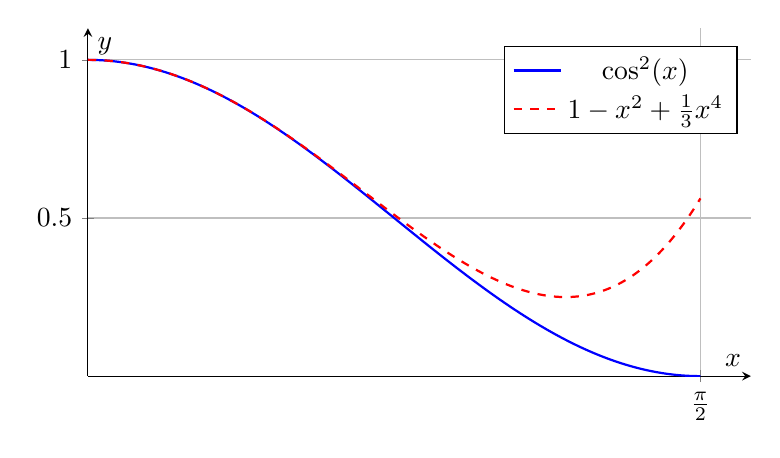
\begin{tikzpicture}
			\begin{axis}[
				domain=0:pi/2,
				samples=200,
				axis lines=middle,
				xlabel={$x$},
				ylabel={$y$},
				xmin=0, xmax=1.7,
				ymin=0, ymax=1.1,
				xtick={0,1.5708},
				xticklabels={$0$, $\frac{\pi}{2}$},
				ytick={0,0.5,1},
				grid=both,
				width=10cm,
				height=6cm,
				legend style={at={(0.98,0.95)},anchor=north east}
				]
				% cos^2(x)
				\addplot[thick,blue] {cos(deg(x))^2};
				\addlegendentry{$\cos^2(x)$}
				
				% 1 + x^2 + x^4
				\addplot[thick,red,dashed] {1 - x^2 + 0.3333333*x^4};
				\addlegendentry{$1 - x^2 + \frac{1}{3}x^4$}
			\end{axis}
		\end{tikzpicture}
		\caption{\textit{The blue continuous line is the function we want to integrate, $f(x)= \cos^2(x)$. The red dotted line is the proposal $g(x) = 1+bx^2+cx^4$ (unnormalized) where $b = -1, c = \frac{1}{3}$}}
		\label{fig:figref}
	\end{figure}
	\newpage
	\section{Lecture 4: Markov chains}
	\subsection{Exercise 1}
	The state probability vector of a Markov chain $\mu_n$ satisfies the recurrence relation:
	\begin{equation}
		\mu_n = \mu_{n-1} \textbf{P}
		\label{eq:mastereq}
	\end{equation}
	
	Show that this equation is equivalent to writing
	$$
	\mu_n(i) = \Bigl(1-\sum_{j\neq i}p_{ji}\Bigr)\mu_{n-1}(i)+\sum_{j\neq i}p_{i,j}\mu_{n-1}(j)
	$$
	Explain the meaning of this equation in terms of a dynamical equation for the state vector.
	\textbf{\\Resolution\\}
	Let's start by rewriting Eq.\ref{eq:mastereq} by elements:
	$$
	\mu_n(i) = \sum_{j\in S}\mu_{n-1}(j)p_{ji} = \sum_{j\neq i}\mu_{n-1}(j)p_{ji}+ \mu_{n-1}(i)p_{ii}
	$$
	To ensure probability conservation, $\textbf{P}$ must be stochastic, i.e. normalized across rows:
	$$
	\sum_{j}p_{i,j} = 1 = p_{ii}+\sum_{j\neq i}p_{i,j} 
	$$
	substituing $p_{ii}$ into the previous formulae, we get:
	$$
	\mu_n(i) = \sum_{j\in S}\mu_{n-1}(j)p_{ji} = \sum_{j\neq i}\mu_{n-1}(j)p_{ji}+ \mu_{n-1}(i)(1 - \sum_{j\neq i}p_{i,j}  )
	$$
	$$
	\mu_n(i) = \mu_{n-1}(i)\Bigl(1 - \sum_{j\neq i}p_{i,j}\Bigr) + \sum_{j\neq i}\mu_{n-1}(j)p_{ji} 
	$$
	The first term can be interpreted as follows. Since $p_{ij}$ represents the probability of transitioning from state $i$ to state $j$, the quantity $\sum_{j\neq i}p_{i,j}$ is just the probability (in the time quanta $\Delta t = 1$) of transitioning to any state $j$ different than the starting state $i$. Therefore the first term simply represents the contribution to the probability of being in state $i$ at time $n-1$ ($\mu_{n}(i)$) due to just standing there, i.e. no transitions has occurred from $n-1$ to $n$. The second term, of course, represents the contribution due to the flux coming from all other states different from $i$ itself. Each state $j\neq i$ will contribute with a factor $p_{ji}\mu_{n-1}(j)$, i.e. the probability of being in $j$ at time $n-1$ times the probability of transitioning from $j$ to $i$.
	
	\subsection{Exercise 2}
	Classify the following Markov chain $\textbf{P}$ in terms of its digraph (to be drawn), irreducibility, and aperiodicity
	\begin{equation}
		\textbf{P} = 
		\begin{pmatrix}
			0.3 & 0.7 & 0 \\
			0.2 & 0.4 & 0.4 \\
			0 & 0.6 & 0.4
		\end{pmatrix}
	\end{equation}
	\textbf{\\Resolution\\}
	The digraph for this Markov process is drawn in Fig.\ref{fig:markov1}.
	\begin{itemize}
		\item The Markov chain $\textbf{P}$ is homogeneous (it does not depend on time)
		\item The Markov chain $\textbf{P}$ is irreducible, since we can reach all of the three states starting from an arbitrary one. State $2$ and $1$ are directly connected and states $3,1$ can be joined together passing by $2$.
		\item The Markov chain $\textbf{P}$ is aperiodic. In fact, starting from each state at time $t=0$, then $\tau = 1$ is always a valid return time thanks to the presence of the non-zero loops. Therefore, the period for each state (the gcd between all return times) is simply $1$ and the chain is aperiodic. Since $\textbf{P}$ is also irreducible, then it is also regular
	\end{itemize}
	\begin{figure}
		\centering
		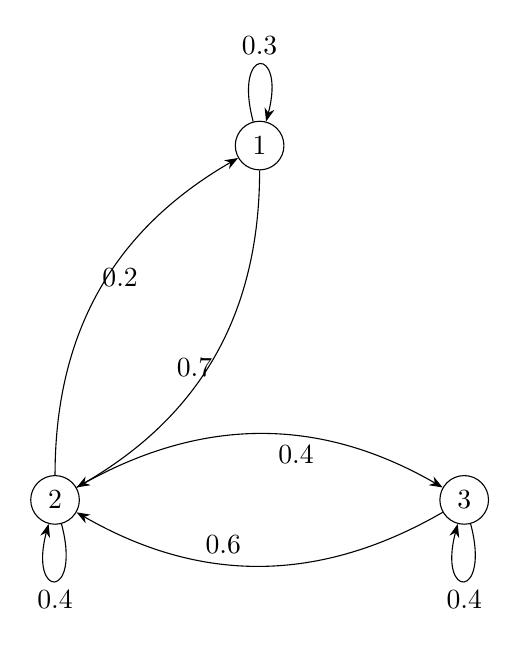
\begin{tikzpicture}[->, >=Stealth, node distance=3cm, every loop/.style={min distance=10mm, looseness=10}]
			% Circular placement
			\node[circle, draw] (1) at (90:3cm) {1};
			\node[circle, draw] (2) at (210:3cm) {2};
			\node[circle, draw] (3) at (330:3cm) {3};
			
			% Edges from 1
			\draw (1) edge[loop above] node[above] {0.3} (1);
			\draw (1) edge[bend left] node[above,pos=0.6] {0.7} (2);
			
			% Edges from 2
			\draw (2) edge[bend left] node[below,pos=0.6] {0.2} (1);
			\draw (2) edge[loop below] node[below] {0.4} (2);
			\draw (2) edge[bend left] node[below,pos=0.6] {0.4} (3);
			
			% Edges from 3
			\draw (3) edge[bend left] node[above,pos=0.6] {0.6} (2);
			\draw (3) edge[loop below] node[below] {0.4} (3);
		\end{tikzpicture}
		\hspace{20pt}
		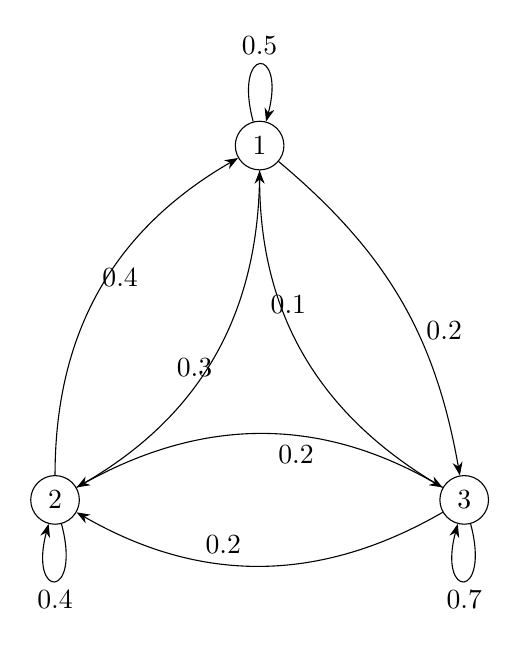
\begin{tikzpicture}[->, >=Stealth, node distance=3cm, every loop/.style={min distance=10mm, looseness=10}]
			% Circular placement
			\node[circle, draw] (1) at (90:3cm) {1};
			\node[circle, draw] (2) at (210:3cm) {2};
			\node[circle, draw] (3) at (330:3cm) {3};
			
			% Edges from 1
			\draw (1) edge[loop above] node[above] {0.5} (1);
			\draw (1) edge[bend left] node[above,pos=0.6] {0.3} (2);
			\draw (1) edge[bend left=20] node[right,pos=0.6] {0.2} (3);
			
			% Edges from 2
			\draw (2) edge[bend left] node[below,pos=0.6] {0.4} (1);
			\draw (2) edge[loop below] node[below] {0.4} (2);
			\draw (2) edge[bend left] node[below,pos=0.6] {0.2} (3);
			
			% Edges from 3
			\draw (3) edge[bend left] node[above,pos=0.6] {0.1} (1);
			\draw (3) edge[bend left] node[above,pos=0.6] {0.2} (2);
			\draw (3) edge[loop below] node[below] {0.7} (3);
		\end{tikzpicture}
		\caption{\textit{Markov chain as digraphs, exercises 1 and 2}}
		\label{fig:markov1}
	\end{figure}
	
	\subsection{Exercise 3}
	Find the fixed points of the following Markov chain and determine if they are unique.
	\begin{equation}
		\textbf{P} = 
		\begin{pmatrix}
			0.5 & 0.3 & 0.2 \\
			0.4 & 0.4 & 0.2 \\
			0.1 & 0.2 & 0.7
		\end{pmatrix}
	\end{equation}
	The Markov chain (right panel of Fig.\ref{fig:markov1}) is homogeneous and irreducible, since any state is reachable from any other states. Again, thanks to the non-zero loops, the chain is also aperiodic, thus it's regular
	
	If a Markov chain is regular, then we know there exists a unique invariant distribution $\vec{\pi}$ to which any initial state converges. It can be found by imposing:
	$$
	\vec\pi = \vec\pi \textbf{P}
	$$ 
	\begin{equation}
		\begin{pmatrix}
			\pi_1 & \pi_2 & \pi_3
		\end{pmatrix} =  \begin{pmatrix}
			\pi_1 & \pi_2 & \pi_3
		\end{pmatrix}
		\begin{pmatrix}
			0.5 & 0.3 & 0.2 \\
			0.4 & 0.4 & 0.2 \\
			0.1 & 0.2 & 0.7
		\end{pmatrix}
	\end{equation}
	\begin{equation}
		\begin{pmatrix}
			\pi_1 & \pi_2 & \pi_3
		\end{pmatrix} = 
		\begin{pmatrix}
			0.5\pi_1 + 0.4\pi_2+0.1\pi_3 & 0.3\pi_1 + 0.4\pi_2+0.2\pi_3 & 0.2\pi_1 + 0.2\pi_2+0.7\pi_3
		\end{pmatrix}
	\end{equation}
	\begin{equation}
		\begin{cases}
			-0.5\pi_1 + 0.4\pi_2+0.1\pi_3 &= 0 \\
			0.3\pi_1 - 0.6\pi_2+0.2\pi_3 &=0 \\
			0.2\pi_1 + 0.2\pi_2-0.3\pi_3 &=0
		\end{cases}
	\end{equation}
	The normalized solution is:
	$$
	\pi_1 = \frac{14}{45} \quad \pi_2 = \frac{13}{45} \quad \pi_3 = \frac{18}{45}
	$$
	\subsection{Exercise 4}
	Determine if the following Markov chain $\textbf{P}$ is irreducible and aperiodic, and find its period if it is not aperiodic:
	\begin{equation}
		\textbf{P} = 
		\begin{pmatrix}
			0 & 1 & 0 & 0 \\
			0.5 & 0 & 0.5 & 0 \\
			0 & 0 & 0 & 1 \\
			0 & 0.5 & 0 & 0.5
		\end{pmatrix}
	\end{equation}
	\textbf{\\Resolution\\}
	The digraph is represented in Fig.\ref{fig:mark2}. The markov chain is irreducible: it's possible to go from any node to any other nodes. Regarding the period, let's take as an example the state $1$. Starting from there, the possible return times are $2$ ($1\to2\to1$), $4$ ($1\to2\to1\to2\to1$), $5$ ($1\to2\to3\to4\to2\to1$), thus the gdc is $1$.
	Node $4$ has for sure period $1$ thanks to the loop. Node $3$ has return times $3$($3\to4\to2\to3$), $4$ ($3\to4\to4\to2\to3$) thanks again to the loop, so the gdc is $1$ again. The same logic goes on for node $2$, since we can travel from node $2$ to node $4$ and loop over it an arbitrary amount of time. Therefore, all nodes have period $1$ and the Markov chain is aperiodic
	\begin{figure}
		\centering
		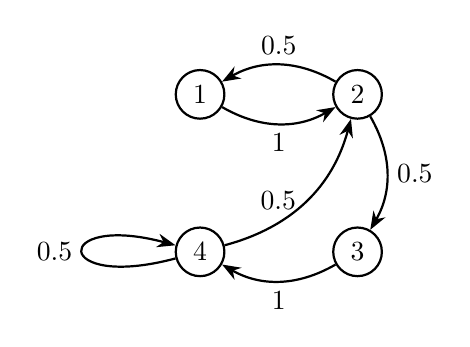
\begin{tikzpicture}[->, >=Stealth, 
			every loop/.style={min distance=10mm, looseness=25},
			node distance=5cm, thick]
			
			% Nodi disposti ai vertici di un quadrato
			\node[circle, draw] (1) at (0,2) {1};
			\node[circle, draw] (2) at (2,2) {2};
			\node[circle, draw] (3) at (2,0) {3};
			\node[circle, draw] (4) at (0,0) {4};
			
			% --- Transizioni non nulle secondo la matrice P ---
			% Da 1
			\draw (1) edge[bend right] node[below]{1} (2);
			
			% Da 2
			\draw (2) edge[bend left] node[right]{0.5} (3);
			\draw (2) edge[bend right] node[above]{0.5} (1);
			
			% Da 3
			\draw (3) edge[bend left] node[below]{1} (4);
			
			% Da 4
			\draw (4) edge[bend right] node[left]{0.5} (2);
			\draw (4) edge[loop left] node[left]{0.5} (4);
		\end{tikzpicture}
		\hspace{10pt}
		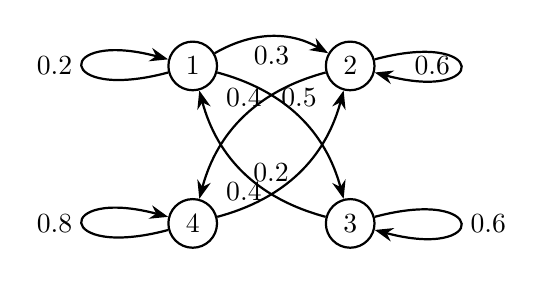
\begin{tikzpicture}[->, >=Stealth, 
			every loop/.style={min distance=15mm, looseness=20},
			node distance=7cm, thick]
			
			% Nodi disposti ai vertici di un quadrato
			\node[circle, draw] (1) at (0,2) {1};
			\node[circle, draw] (2) at (2,2) {2};
			\node[circle, draw] (3) at (2,0) {3};
			\node[circle, draw] (4) at (0,0) {4};
			
			% --- Transizioni non nulle secondo la matrice P ---
			% Da 1
			\draw (1) edge[loop left] node[left]{0.2} (1);
			\draw (1) edge[bend left] node[below]{0.3} (2);
			\draw (1) edge[bend left] node[above]{0.5} (3);
			
			
			% Da 2
			\draw (2) edge[loop right] node[left]{0.6} (2);
			\draw (2) edge[bend right] node[above]{0.4} (4);
			
			% Da 3
			\draw (3) edge[bend left] node[below]{0.4} (1);
			\draw (3) edge[loop right] node[right]{0.6} (3);
			
			% Da 4
			\draw (4) edge[bend right] node[left]{0.2} (2);
			\draw (4) edge[loop left] node[left]{0.8} (4);
		\end{tikzpicture}
		\hspace{10pt}
		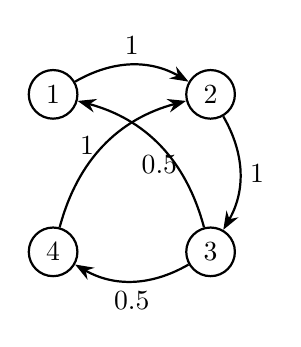
\begin{tikzpicture}[->, >=Stealth, 
			every loop/.style={min distance=15mm, looseness=20},
			node distance=7cm, thick]
			
			% Nodi disposti ai vertici di un quadrato
			\node[circle, draw] (1) at (0,2) {1};
			\node[circle, draw] (2) at (2,2) {2};
			\node[circle, draw] (3) at (2,0) {3};
			\node[circle, draw] (4) at (0,0) {4};
			
			% --- Transizioni non nulle secondo la matrice P ---
			% Da 1
			\draw (1) edge[bend left] node[above]{1} (2);
			
			
			% Da 2
			\draw (2) edge[bend left] node[right]{1} (3);
			
			% Da 3
			\draw (3) edge[bend right] node[below]{0.5} (1);
			\draw (3) edge[bend left] node[below]{0.5} (4);
			
			% Da 4
			\draw (4) edge[bend left] node[left]{1} (2);
		\end{tikzpicture}
		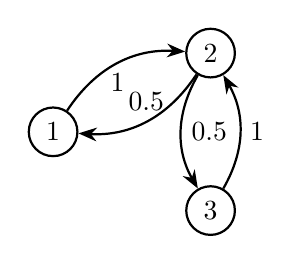
\begin{tikzpicture}[->, >=Stealth, 
			every loop/.style={min distance=15mm, looseness=20},
			node distance=7cm, thick]
			
			% Nodi disposti ai vertici di un quadrato
			\node[circle, draw] (1) at (0,1) {1};
			\node[circle, draw] (2) at (2,2) {2};
			\node[circle, draw] (3) at (2,0) {3};
			
			% --- Transizioni non nulle secondo la matrice P ---
			% Da 1
			\draw (1) edge[bend left] node[below]{1} (2);
			
			
			% Da 2
			\draw (2) edge[bend left] node[above]{0.5} (1);
			\draw (2) edge[bend right] node[right]{0.5} (3);
			
			% Da 3
			\draw (3) edge[bend right] node[right]{1} (2);
			
		\end{tikzpicture}
		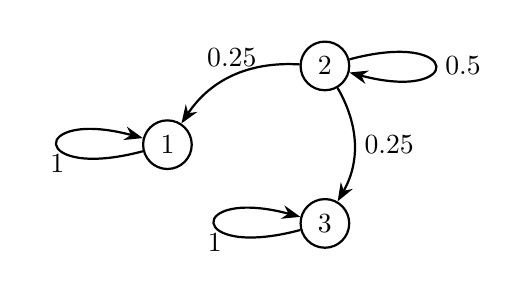
\begin{tikzpicture}[->, >=Stealth, 
			every loop/.style={min distance=15mm, looseness=20},
			node distance=7cm, thick]
			
			% Nodi disposti ai vertici di un quadrato
			\node[circle, draw] (1) at (0,1) {1};
			\node[circle, draw] (2) at (2,2) {2};
			\node[circle, draw] (3) at (2,0) {3};
			
			% --- Transizioni non nulle secondo la matrice P ---
			% Da 1
			\draw (1) edge[loop left] node[below]{1} (1);
			
			
			% Da 2
			\draw (2) edge[bend right] node[above]{0.25} (1);
			\draw (2) edge[loop right] node[right]{0.5} (2);
			\draw (2) edge[bend left] node[right]{0.25} (3);
			
			% Da 3
			\draw (3) edge[loop left] node[below]{1} (3);
			
		\end{tikzpicture}
		\caption{\textit{(Top Left) Markov chain digraph for exercise 4 (Top Right) Markov chain digraph for exercise 5 (Bottom Left) Markov chain digraph for exercise 6 (Bottom center) Markov chain digraph for exercise 7 (Bottom right) Markov chain digraph for exercise 8}}
		\label{fig:mark2}
	\end{figure}
	
	\subsection{Exercise 5}
	Determine if the following Markov chain $\textbf{P}$ is irreducible and aperiodic, and find its period if it is not aperiodic:
	\begin{equation}
		\textbf{P} = 
		\begin{pmatrix}
			0.2 & 0.3 & 0.5 & 0 \\
			0 & 0.6 & 0 & 0.4 \\
			0.4 & 0 & 0.6 & 0 \\
			0 & 0.2 & 0 & 0.8
		\end{pmatrix}
	\end{equation}
	\textbf{\\Resolution\\}
	The digraph is represented in Fig.\ref{fig:mark2}. The markov chain isn't irreducible: in fact, you can't go from node $2$ to node $1$ or node $3$
	
	Regarding the period, the presence of self-loops implies that each node has period $1$, so the Markov chain as a whole is aperiodic.
	
	\subsection{Exercise 6}
	Draw the digraph corresponding to the following stochastic matrix:
	\begin{equation}
		\textbf{P} = 
		\begin{pmatrix}
			0 & 1 & 0 & 0 \\
			0 & 0 & 1 & 0 \\
			0.5 & 0 & 0 & 0.5 \\
			0 & 1 & 0 & 0
		\end{pmatrix}
	\end{equation}
	Is the corresponding Markov chain irreducible? Is periodic? If yes, compute the corresponding period
	\textbf{\\Resolution\\}
	The digraph is represented in Fig.\ref{fig:mark2}. It is irreducible, since we can reach any states starting from any arbitrary initial states. Regarding the period,
	\begin{itemize}
		\item Starting from state $1$, the Markov chain necessarily continues to state $2$ and then $3$. From node $3$, we can return to state $1$ (return time of $3$) or continue to state $4$. From node $4$, the only way out is to transition to node $2$ and again $3$, for a total of $3$ more steps. Hence, the period of node $1$ is $3$
		\item Since the chain is irreducible, all states will have period $3$
	\end{itemize}
	In conclusion, this Markov chain is irreducible but periodic with period $3$.
	\subsection{Exercise 7}
	Determine if the following Markov chain is irreducible and aperiodic, and find its period if it is not aperiodic. Show it by using both the digraph and the matrix.
	\begin{equation}
		\textbf{P} = 
		\begin{pmatrix}
			0 & 1 & 0  \\
			0.5 & 0 & 0.5\\
			0 & 1 & 0 
		\end{pmatrix}
	\end{equation}
	The Markov chain is irreducible, any state is reachable starting from any other state. Regarding the period,
	\begin{itemize}
		\item Let's start in node $1$. We are forced to transition to node $2$. From here, we can return in node $1$ (return time of $2$) or migrate to node $3$. From node $3$, we must return to node $2$ and if we want to get back in node $1$, we would do so with a return time of $4$. It's easy to show that the all return times of state $1$ must be even, so the its period is $2$.
		\item Since the chain is irreducible, all states will have period $2$. Therefore the chain as a whole is not aperiodic (and has period $2$).
	\end{itemize}
	We can prove the same result using the matrix representation of the Markov chain. In fact, it's easy to show that:
	\begin{equation}
		\begin{pmatrix}
			0 & 1 & 0  \\
			0.5 & 0 & 0.5\\
			0 & 1 & 0 
		\end{pmatrix}^{2n+1} = \begin{pmatrix}
			0 & 1 & 0  \\
			0.5 & 0 & 0.5\\
			0 & 1 & 0 
		\end{pmatrix}
	\end{equation}
	thus $(\textbf{P}^{2n+1})_{ii} = 0, \forall i$, meaning that the probability to start from $i$ and be back in $i$ at time $t = 2n+1$ is zero if $t$ is odd. Therefore, return times must be even and the period is $2$.
	\subsection{Exercise 8}
	Draw the digraph related to the following Markov Matrix
	\begin{equation}
		\textbf{P} = 
		\begin{pmatrix}
			1 & 0 & 0  \\
			\frac{1}{4} & \frac{1}{2} & \frac{1}{4} \\
			0 & 0 & 1 
		\end{pmatrix}
	\end{equation}
	Show that this Markov chain has more than one stationary distribution and find to which limiting matrix of $\textbf{P}^n$ as $n\to\infty$
	\textbf{\\Resolution\\}
	The digraph is shown in Fig.\ref{fig:mark2}. It's quite easy to verify that $1$ is an absorbing state since $p_{1,1} = 1$, therefore the chain is not irreducible (it's not possible to start in $1$ and end anywhere else). The same reasoning goes for node $3$.
	
	Since all three nodes have non-zero self-loops, then the Markov chain is aperiodic, but since it's not irreducible, we can't claim it is also regular. This means that we don't have any guarantee on the uniqueness and existence of the invariant distribution $\vec\pi$. Solving for $\vec\pi$ as we did in Exercise 3, we obtain the linear system:
	\begin{equation}
		\begin{cases}
			0.25\pi_2 &= 0 \\
			- 0.5\pi_2 &=0 \\
			-0.75\pi_2 &=0
		\end{cases}
	\end{equation}
	and any generic normalized state $\vec{\pi} = (p, 0, 1-p)$ is a valid invariant distribution. This is reasonable, since states $1$ and $3$ are absorbing: if $\vec\mu_0 = \delta_{n,1}$, the system will converge to $\vec\pi = \delta_{n,1}$ (it will just stay there), and the same goes when $\vec\mu_0 = \delta_{n,3}$ that will converge to itself. To better understand this behaviour, let's eigen decompose the matrix $\textbf{P}$:
	\begin{equation}
		\mathbf{P} = \mathbf{Q}\mathbf{\Pi}\mathbf{Q}^{-1} = 
		\begin{pmatrix}
			0 & -1 & 2 \\
			1 & 0 & 1 \\
			0 & 1 & 0
		\end{pmatrix}
		\begin{pmatrix}
			0.5 & 0 & 0 \\
			0 & 1 & 0 \\
			0 & 0 & 1
		\end{pmatrix}
		\begin{pmatrix}
			-0.5 & 1 & -0.5 \\
			0 & 0 & 1 \\
			-0.5 & 0 & 0.5
		\end{pmatrix}
	\end{equation}
	And, as expected, the eigenvalue $\lambda = 1$, the one defining the invariant distribution, is degenerate. Now since $\textbf{P}^n = \mathbf{Q} \mathbf{\Pi}^n \mathbf{Q}^{-1}$ and $(0.5)^{\infty} \to 0$, then:
	\begin{equation}
		\vec\pi = \lim_{n\to\infty} \vec{\mu}_0 \textbf{P}^n = \vec{\mu}_0 \textbf{Q}
		\begin{pmatrix}
			0 & 0 & 0 \\
			0 & 1 & 0 \\
			0 & 0 & 1
		\end{pmatrix} \textbf{Q}^{-1} = \vec\mu_0 \begin{pmatrix}
			1 & 0 & 0 \\
			0.5 & 0 & 0.5 \\
			0 & 0 & 1
		\end{pmatrix} = (p_1^{(0)}+0.5p_2^{(0)}, 0, 0.5p_2^{(0)} + p_3^{(0)})
	\end{equation}
	which is precisely what we expect (up to a normalization factor). The stationary value of $\pi_2$ is $0$, since once state $2$ is exited it is never to be returned. All the probability will be split between the two absorbing states depending on the initial condition. In fact, rewriting  $p_2^{(0)} = 1 - p_1^{(0)}-p_3^{(0)}$, we obtain:
	\begin{equation}
		\begin{cases}
			\pi_1 = \frac{1}{2} (1 + p_1^{(0)} -   p_3^{(0)}) \\
			\pi_2 = 0\\
			\pi_3 =  \frac{1}{2} (1 + p_3^{(0)} -   p_1^{(0)})
		\end{cases}
	\end{equation}
	
	\subsection{Exercise 9}
	Find the matrix of a Markov chain describing a biased random walk in two dimensions ($d=2$), where the bias is along the positive x-axis, and its stationary distribution.
	\textbf{\\ Resolution \\}
	We are going to assume that the random walker makes a move every $\Delta t$ seconds. At each step, the walker independently moves both in the horizontal and vertical direction by a discrete amount $\Delta r$, so that the topology is effectively $\mathbb{Z}$ and we can label each lattice point with an integer pair $(i,j)$ (and two consecutive points are a distance $\Delta r$ away from each other). The walker has no bias in the vertical direction, so it can go up or down with the same probability $1/2$. At variance, we must impose a bias in the horizontal direction: at each $\Delta t$, the walker will move to the right with probability $p$ and to the left with probability $1-p$. 
	
	We can to describe this process through a discrete-time discrete-state space Markov chain. Since the space state is infinite, there's no finite matrix representation of the process, however we can at least write the transition rates $p_{(ij), (i',j')}$, i.e. the probability that the walker will transition from $(i,j)$ to $(i',j')$ in $\Delta t$ time units. Imposing the bias condition,
	\begin{equation}
		p_{(ij), (i',j')} = 
		\begin{cases}
			\frac{1}{2}p \quad\mbox{    if }  (i',j') = (i+1, j\pm 1) \\
			\frac{1}{2}(1-p) \quad\mbox{    if }  (i',j') = (i-1, j\pm 1) \\
		\end{cases}
	\end{equation}
	Because at each step the horizontal and vertical move are statistically independent, we can consider this motion as two separate one-dimensional random walkers. When the number of steps $N$ grows to infinity (or when $\Delta r, \Delta t \to 0$), we can invoke the central limit theorem and claim that:
	\begin{equation}
		\begin{aligned}
			p(x) \approx \frac{1}{\sigma_x\sqrt{2\pi N}}\exp\Bigl(-\frac{(x-\mu_x)^2}{2N\sigma_x^2}\Bigr)  \\
			p(y) \approx \frac{1}{\sigma_y\sqrt{2\pi N}}\exp\Bigl(-\frac{(y-\mu_y)^2}{2N\sigma_y^2}\Bigr)
		\end{aligned}
	\end{equation}
	where $x,y$ are integer value. The statistical quantities $\mu_x, \mu_y, \sigma_x, \sigma_y$ are related to a single stochastic step in the $x$ or $y$ direction:
	\begin{equation}
		\begin{aligned}
			\mu_y &= \langle y\rangle = \frac{1}{2}(\Delta r) + \frac{1}{2}(-\Delta r) = 0\\
			\sigma_y^2 &= \langle y^2 \rangle - \langle y \rangle^2 = \frac{1}{2}(\Delta r)^2 + \frac{1}{2}(\Delta r)^2 = \Delta r^2 \\
			\mu_x &= \langle x\rangle = p(\Delta r) + q(-\Delta r) = (p-q) = (2p-1)\Delta r\\
			\sigma_x^2 &= \langle x^2 \rangle - \langle x \rangle^2 = p(\Delta r)^2 + q(-\Delta r)^2 - (p-q)^2\Delta r^2 = (1 - (2p-1)^2)\Delta r
		\end{aligned}
	\end{equation}
	Since the state-space is infinite, there's no proper stationary distribution other than the infinitesimal distribution across all $\mathbb{Z}$. To have a sensible invariant distribution, let's imagine that the random walker is constrained by a square centered in the origin, i.e. $p_{ij} \neq 0$ if $ -L/2 < x < L/2, - L/2 < y < L/2 $, $(N_x, N_y \in \mathbb{N})$ and is $0$ elsewhere. We can't use the central limit theorem anymore because now the steps may be correlated (if the walker is close to the border, there are some forbidden moves). Fortunately, in the continuum limit, this is a classical diffusion problem described by the Fokker-Planck:
	\begin{equation}
		\frac{\partial p (x,y,t)}{\partial t} = -v\frac{\partial p}{\partial x} + D \Bigl( \frac{\partial^2p(x,y,t)}{\partial x^2} +\frac{\partial^2p(x,y,t)}{\partial y^2}\Bigr)
	\end{equation}
	With the proper reflective boundary conditions. The stationary (i.e. invariant) distribution satisfies:
	\begin{equation}
		0 = -v\frac{\partial p}{\partial x} + D \Bigl( \frac{\partial^2p(x,y,t)}{\partial x^2} +\frac{\partial^2p(x,y,t)}{\partial y^2}\Bigr)
	\end{equation}
	This is solved by:
	\begin{equation}
		p(x,y)^* = A \exp\Bigl(\frac{v}{D}x\Bigr) \quad\quad\quad\quad (x,y) \in [-L/2, L/2]^2 
	\end{equation}
	As expected, there is no dependence on $y$. Along the horizontal direction, the probability distribution (in the continuous limit) is exponential and peaks around $x = L/2$, as it should since the drift term will bias towards the border the walker. If $v = 0$, i.e. $p = \frac{1}{2}$, then we obtain back the uniform distribution.
	
	\newpage	
	\section{MC simulation of a 2D Ising model by the Metropolis algorithm}
	Write a program that simulates a 2D Ising model with periodic boundary conditions by using the Metropolis acceptance matric $a_{ij}$ and the matrix $\Gamma_{ij}$ based on the local spin-flip (Glauber) proposed move
	
	\textbf{\\ Resolution \\}
	The code developed to run the MCMC simulation can be found in \href{https://github.com/lorenzorizzi17/YAIS}{this repository}. A snapshot of the C++ function that specifically performs a Monte Carlo step is shown here for the sake of examplification:
	\begin{lstlisting}
		void MCMCengine::MetropolisHastings() {
			std::uniform_int_distribution<int> dist(0, m_N - 1);
			int index = dist(m_rng);
			int L = static_cast<int>(std::sqrt(m_N));
			int row = index / L;
			int col = index % L;
			
			// extract the spin value
			int spin = m_spinConfig->getSpins()[index] ? 1 : -1;
			int neighbourSum = 0;
			std::array<int,4> neighbours = m_spinConfig->getNeighbourhoodSpins(row, col);
			for (int i = 0; i < 4; ++i) {
				neighbourSum += neighbours[i];
			}
			double exponentialFactor = std::exp(- 2* double(spin) * static_cast<double>(neighbourSum) / m_spinConfig->getTemperature() + 2 * m_spinConfig->getMagneticField() * double(spin) / m_spinConfig->getTemperature());
			// Metropolis-Hastings criterion: accept if ...
			if (exponentialFactor > 1.0 || std::uniform_real_distribution<double>(0.0, 1.0)(m_rng) < exponentialFactor) {
				m_spinConfig->getSpins()[index] = !m_spinConfig->getSpins()[index];   
			}
		}
	\end{lstlisting}
	\subsection{Ising model at various temperatures: qualitative analysis}
	By assuming $k_B = 1$ and $J = 1$, we simulate the 2D Ising model for different values of temperature and three different values of $L$ (the linear size of the lattice). In this specific case, we will choose: $L = 100, 200, 500$ and $T = 1, 2.26, 4$ (assuming $k_B=1$ and $J=1$, so temperatures are dimensionless). A snapshot for each combination of size and temperature is shown in Fig.~\ref{fig:ising1}, Fig.~\ref{fig:ising2}, and Fig.~\ref{fig:ising3}.
	
	When $T = 4$, the temperature is well above the critical value $T_c = \frac{2}{\ln(1+\sqrt{2})}\approx 2.26$ (Onsager), and the system should always relax to a disordered phase where the average magnetization is zero (at least in the thermodynamic limit), regardless of the initial configuration. This is precisely what we observe running our Metropolis algorithm: when $T = 4$, the system looks fuzzy (left panels of Fig.~\ref{fig:ising1}, Fig.~\ref{fig:ising2}, Fig.~\ref{fig:ising3}) and the spins are oriented up or down in a seemingly equiprobable fashion. Macroscopically, the system lies in a disordered phase, where the entropic contribution prevails over the energy term.
	
	When $T = 1$, the temperature is well below the critical point, and the system should display an ordered ferromagnetic phase according to our understanding of the Ising model. In the thermodynamic limit, two equilibrium states appear with opposite average magnetization, $m_1(T) = -m_2(T)$. In this specific case, the initial condition will determine to which of these equilibrium ordered phases\footnote{This is not strictly true, especially when the size of the system is not large enough, the algorithm will explore both equilibrium macrostates. A more detailed discussion will follow up later} the system will converge, depending on the initial percentage of up spins versus down spins (spontaneous breaking of symmetry). In the simulations I ran, I selected the initial configuration such that approximately $60\%$ of the spins pointed up (blue), and thus we observe a symmetry breaking towards a macroscopic ordered phase where most of the spins are up (in agreement with the right panels of Fig.~\ref{fig:ising1}, Fig.~\ref{fig:ising2}, Fig.~\ref{fig:ising3}).
	
	Finally, when $T = 2.26 \approx T_c$, the system exhibits peculiar properties. Around criticality, we know that the model takes a long time to thermalize, and consequently, the MC Markov chain requires a huge number of steps to reach the desired invariant distribution (the Boltzmann one). Therefore, one cannot be completely sure that the snapshots in Fig.~\ref{fig:ising1}, Fig.~\ref{fig:ising2}, and Fig.~\ref{fig:ising3} (central panels) truly represent samples drawn from the equilibrium Boltzmann distribution of the Ising model. From the theory of phase transitions, we also know that, at criticality, the correlation length diverges\footnote{This is strictly true only in the thermodynamic limit, i.e., for an infinite system. Our simulations are, of course, finite, so the correlation length will simply reach a maximum and then decrease again.}. This means that spins will tend to create \textit{correlated clusters} whose size is of the same order as the correlation length (diverging at $T_c$), i.e., the system will appear as a mix of mesoscopic ordered phases that take a long time to thermalize with each other. These clusters can be easily seen in the central panels of Fig.~\ref{fig:ising1}, Fig.~\ref{fig:ising2}, and Fig.~\ref{fig:ising3}.
	
	\begin{figure}
		\centering
		\includegraphics[scale = 0.17]{fig/100_4.png}
		\includegraphics[scale = 0.17]{fig/100_226.png}
		\includegraphics[scale = 0.17]{fig/100_1.png}
		\caption{\textit{Snapshots from the simulations when $L = 100$ (thus $N = 100^2$) for three different values of (starting from the left) $T = 4, T = 2.26, T = 1$ }}
		\label{fig:ising1}
	\end{figure}
	\begin{figure}
		\centering
		\includegraphics[scale = 0.17]{fig/200_4.png}
		\includegraphics[scale = 0.17]{fig/200_226.png}
		\includegraphics[scale = 0.17]{fig/200_1.png}
		\caption{\textit{Snapshots from the simulations when $L = 200$ (thus $N = 200^2$) for three different values of (starting from the left) $T = 4, T = 2.26, T = 1$}}
		\label{fig:ising2}
	\end{figure}
	\begin{figure}
		\centering
		\includegraphics[scale = 0.17]{fig/500_4.png}
		\includegraphics[scale = 0.17]{fig/500_226.png}
		\includegraphics[scale = 0.17]{fig/500_1.png}
		\caption{\textit{Snapshots from the simulations when $L = 500$ (thus $N = 500^2$) for three different values of (starting from the left) $T = 4, T = 2.26, T = 1$}}
		\label{fig:ising3}
	\end{figure}
	
	\subsection{Time behaviour of the order parameter}
	By showing the time behaviour (in MC steps) of both the order parameter (magnetization per spin) and the energy density discuss what is happening above, below and close
	to the transitions. How can we establish that the Markov chain is sampling according to the desired probability distribution independent on the initial conditions?
	
	\textbf{\\ Resolution \\}
	Let us fix the lattice size $L = 500$ (thus total number of spins $N = 500^2$). Fig.~\ref{fig:23} shows the trace plot (that is, the random walk of the MC chain) and the final histogram for both the average magnetization per spin $m$ and the energy per spin $\epsilon$ when $T = 4$ and when $T=1$, i.e., far from the critical point. As one can easily observe, both equilibrium distributions for $m$ and $\epsilon$ resemble a normal distribution whose average value represents the thermodynamic value at that temperature (and the variance should decrease as $N \to \infty$). How can we establish whether the Markov chain has actually converged to the target distribution, i.e., the Boltzmann distribution? There are many ways to ensure that the Markov chain has reached stationarity. The most important property of an invariant distribution is that it is asymptotically reached independently of the initial condition. This means that one could repeat the same MCMC simulation with a different initial starting configuration and compare the results. If the final distribution looks the same independently of the specific choice of the initial configuration, then we have probably succeeded in sampling from the correct Boltzmann distribution. This was implemented in the code by launching a multi-threaded set of chains where each thread receives different initial configuration and by comparing the final distributions.
	
	Another way to get a sense of the stationarity of the Markov chain is by closely examining the trace plot of the chain. Fig.~\ref{fig:23} shows desirable and clear trace plots for both $m$ and $\epsilon$. The dependence on the initial condition is quickly damped (the abrupt drop observed in the magnetization trace plots), and the algorithm remains in a well-defined region of the $m$ (or $\epsilon$) space, exploring, however, nicely the distribution space.
	
	A different scenario appears when $T$ is close to the critical value ($T = 2.26$, Fig.~\ref{fig:235}). Now the magnetization trace plot clearly looks like it hasn't yet reached a plateau, and the algorithm was probably still exploring the space when it reached the inputted maximum number of MC steps. This is to be expected: around criticality, MCMC algorithms that use local moves suffer from \textit{critical slowing down}, meaning that they take a huge number of steps to finally reach the invariant distribution. Computing statistical averages on those histograms is problematic, since the system has not reached equilibrium and any thermodynamic average would make no physical sense. Why does this happen? The critical slowing down of the MCMC algorithm is related, once again, to the diverging property of the correlation length $\epsilon$ around the critical point. As we have already claimed before, around $T_c$ bubbles of correlated spins will start to appear; out of criticality, those correlated clusters are usually small, but when approaching $T\to T_c$ their size diverges according to a power law. Take again the example of a 2D spin system where one spin has four nearest neighbors when $T \approx T_c$. If this spin is surrounded by aligned spins, its contribution to the energy is $E = -4$ and after the reversal of this spin, this becomes $E = 4$, thus a $\Delta E$ associated to the spin flip of $8$. Right at $T_c$, the acceptance probability is low for the Metropolis algorithm: $ A(s\to s') = \exp(-8/T_c) = 0.0294$: most of the flipping attempts are rejected. Only spin flips at the edge of a cluster have a significant effect over a longer time; but their fraction becomes vanishingly small when the critical temperature is approached and the cluster size diverges. Hence, the critical divergence of $\epsilon$ is directly tied to the inefficiency of our sampling algorithm at criticality\footnote{To sample efficiently when $T \approx T_c$, one should use MC proposal moves that flip entire clusters of spin (Wolff algorithm)}
	
	An interesting phenomena that was observed is that, in general, the average energy per spin $\langle \epsilon \rangle$ has much nicer convergence properties than the magnetization per spin $\langle m \rangle$. This is particularly evident in Fig.\ref{fig:235}, where it's easy to see how the MC chain associated to $m$ is still struggling to find the desired invariant distribution after $2000$ MC steps, whereas the chain associated to $\langle \epsilon\rangle$ has nicely found its equilibrium distribution after just $\approx 500$ MC steps. 
	\begin{figure}
		\centering
		\hspace{-1cm}
		\includegraphics[width=0.52\linewidth]{fig/magnetization_N250000_T4.00_H0.00_t2000_th5.pdf}
		\includegraphics[width=0.52\linewidth]{fig/magnetization_N250000_T1.00_H0.00_t2000_th5.pdf}
		
		\hspace{-3cm}
		\includegraphics[width=0.52\linewidth]{fig/energy_N250000_T4.00_H0.00_t2000_th5.pdf}
		\includegraphics[width=0.52\linewidth]{fig/energy_N250000_T1.00_H0.00_t2000_th5.pdf}
		\hspace{-2cm}
		\caption{\textit{(Top Left) Histograms and trace plots, i.e. collected samples of the MCMC over time, for the average magnetization $m$ (top sector) and for $\epsilon$ (bottom sector) when $N = 500^2, T = 4$ (left sector) and $T = 1$ (right sector). The simulation was run until $2000$ samples were collected. The initial configuration was quickly forgotten, as one can see by examining the abrupt drop during the first MC steps. The trace plots correctly moves in the phase space and efficiently explores it, while the histograms closely resemble a Gaussian distribution peaked around the thermodynamic value $\langle m \rangle, \langle \epsilon \rangle$.}}
		\label{fig:23}
	\end{figure}
	
	\begin{figure}
		\centering
		\includegraphics[scale = 0.4]{fig/magnetization_N250000_T2.26_H0.00_t2000_th5.pdf}
		\includegraphics[scale = 0.4]{fig/energy_N250000_T2.26_H0.00_t2000_th5.pdf}
		\caption{\textit{(Top Left) Trace plot for the average magnetization $m$ when $N = 500^2$, $T = 2.26$, and $H = 0$. The simulation was run until $2000$ samples were collected. Because we are close to criticality, the system takes a long time to reach equilibrium (critical slowing down). This can be assessed by looking at the trace plot of the MCMC, whose evolving trend clearly suggests that the algorithm has not yet reached the stationary state, i.e., the Boltzmann distribution.(Top Right) Histogram of the $m$ values (over $2000$ samples), using the same parameters as in the trace plot. These results are not representative, since we are not yet sampling from the correct equilibrium distribution.(Bottom Left) Trace plot for the average energy per spin $\epsilon$ when $N = 500^2$, $T = 1$, and $H = 0$. (Bottom Right) Histogram of the collected $\epsilon$ samples.}}
		\label{fig:235}
	\end{figure}
	\subsection{Equilibration time}
	After having determined the equilibrium time $\tau$ and disregarding the samples for $t < \tau$ estimate the ensemble averages of the magnetization per spin, the energy per spin, and the corresponding fluctuations (specific heat per site and magnetic susceptibility
	per site). Plot their estimates as function of the chosen temperatures and discuss the behaviour of the curves as the linear size of the system L increases.
	\textbf{\\ Resolution \\}
	The procedure of disregarding samples for $t < \tau$ with $\tau$ equilibration time is called \textit{burn-in}; $\tau$ is nothing but the characteristic time it takes for the algorithm to converge to the target Boltzmann distribution. Fig.~\ref{fig:taau} represents the trace plot for a MCMC run with $T = 2$ (under-critical regime) and $N = 100\times 100$: it's quite easy to see that the Markov algorithm takes approximately $\tau_{eq} = 50$ MC steps to reach equilibrium. We can now proceed to estimate the thermal averages over samples satisfying $t > \tau$, in particular the order parameter \textit{magnetization per spin} estimated by:
	$$
	\langle m \rangle \approx \bar{m} =  \frac{1}{T_{max}}\sum_{i = \tau}^{T_{max}} m_i 
	$$
	and the energy per spin:
	$$
	\langle \epsilon \rangle \approx \bar\epsilon = \frac{1}{T_{max}}\sum_{i = \tau}^{T_{max}} \epsilon_i
	$$
	where the summation is performed on all MC steps starting from $\tau$ to $T_{max}$, the maximum MC steps. By extracting the variance, we can also estimate the specific heat per spin and the magnetic susceptibility per spin:
	\begin{equation}
		\begin{aligned}
			\frac{\chi}{N} &= N\frac{Var(m)}{T} = N\frac{\langle m^2 \rangle - \langle m \rangle^2}{T} = N\frac{\frac{1}{T_{max}}\sum_i m_i^2 - \bar{m}^2}{T}\\
			\frac{C}{N} &= N\frac{Var(\epsilon)}{T^2} = N\frac{\langle \epsilon^2 \rangle - \langle \epsilon \rangle^2}{T^2} = N\frac{\frac{1}{T_{max}}\sum_i \epsilon_i^2 - \bar{\epsilon}^2}{T^2}
		\end{aligned}
	\end{equation}
	\begin{figure}
		\centering
		\includegraphics[scale = 0.4]{fig/tau.png}
		\caption{\textit{Trace plot for $m$ when $T = 2$ and $N = 100\times100$. The Metropolis algorithm takes a while to reach stationarity (approximately $\tau_{eq}= 50$ MC steps). After $\tau_{eq}$, the algorithm is finally sampling from the desired distribution and we can start computing the thermal averages we are interested in.}}
		\label{fig:taau}
	\end{figure}
	
	Before showing the results, we need to make a small modification to the definition of the order parameter itself. In fact, one should always remember that, as long as the system size is finite,
	$$
	\langle m \rangle = 0, \>\> \forall T
	$$
	This is because the Ising model enjoys a discrete $\mathbb{Z}_2$ symmetry: the configuration ${\sigma_1, \sigma_2, \ldots, \sigma_N}$ with average magnetization $m$ has the same energy as the flipped configuration ${-\sigma_1, -\sigma_2, \ldots, -\sigma_N}$  with average magnetization $-m$ (discarding borders effect). Therefore, they are equiprobable, since the Boltzmann equilibrium distribution is a function only of the Hamiltonian:
	$$
	P(\vec\sigma) = P(-\vec\sigma)
	$$
	This necessarily implies that averaging over the complete Boltzmann distribution yields $\langle m \rangle = 0$ for any temperature. Indeed, if one inspects the trace plot at $T = 2.3$ for a relatively small system size $N = 50\times50$, a peculiar behaviour appears (Fig.~\ref{fig:traceplotpatho}). The random Glauber dynamics seems to have found two symmetric stable points where the chain spends most of its time ($\langle m \rangle \approx \pm 0.6$). We must stress that what is shown in Fig.~\ref{fig:traceplotpatho} is not due to a convergence problem: the MCMC is effectively sampling from the correct Boltzmann distribution. Since the Metropolis algorithm is ergodic by design, it explores the entire parameter space; and as long as $N$ is finite, there will always be two stable wells (minima of the free energy) with $m_1 = -m_2$. The algorithm will eventually jump from one equilibrium to the other, although the probability of such transitions decreases significantly with system size.
	
	How is it thus possible to observe a non-zero $\langle m \rangle$, especially in the ferromagnetic phase? The point is that, for any finite $N$, no true phase transition occurs and $\langle m \rangle$ is indeed zero for all temperatures (because the Metropolis algorithm is ergodic and, given enough time, it will explore both wells). When one wants to understand what happens in the thermodynamic limit, it is crucial to choose the correct order of the limits:
	\begin{equation}
		\langle m \rangle = \lim_{H\to 0}\lim_{N\to\infty}m(T,H) \neq \lim_{N\to\infty}\lim_{H\to 0} m(T,H) = 0
	\end{equation}
	In the (correct) thermodynamic limit, the system undergoes a \textit{spontaneous symmetry breaking}: even though the model is symmetric under spin reversal, it selects a preferred spin orientation, and consequently $\langle m \rangle$ can become different from zero. The Boltzmann distribution remains symmetric under $\vec\sigma \to -\vec\sigma$, but when $N \to \infty$ the thermal energy required to jump from one ordered phase to its opposite diverges, and thus the system will remain permanently in one of the two regions of the $m$-space, depending on the initial condition (the system is no longer ergodic).
	\begin{figure}
		\centering
		\includegraphics[scale = 0.55]{./fig/magnetization_N2500_T2.30_H0.00_t100000_th1.pdf}
		\caption{\textit{Trace plot and histogram of $m$, average magnetization per spin ($T = 2.3, N = 50\times50$). Metropolis algorithm is ergodic, hence it will explore all of the parameter space. When $N$ is finite, the amount of energy needed to jump from one equilibrium state to the other is finite and decreases when $N$ decreases. Thus, especially for small $N$, our algorithm will explore both equilibria, resulting in a bimodal distribution and in a zero average magnetization.}}
		\label{fig:traceplotpatho}
	\end{figure}
	However, our simulations are clearly finite and the thermodynamic limit is unreachable. To avoid averaging over chains such as the one in Fig.~\ref{fig:traceplotpatho} (which would yield an incorrect value of $m$), we can redefine our order parameter as $\langle |m| \rangle$, so that the sign of $m$ becomes irrelevant\footnote{A different approach would have been to introduce a small magnetic field $H$.}. Results are shown in Fig.~\ref{fig:results}. As one would expect, the plot of the average magnetization per spin $\langle m \rangle$ displays what appears to be a second-order phase transition somewhere in the interval $2 < T < 2.5$ (and indeed, we know the exact critical temperature to be $T_c \approx 2.26$ thanks to Onsager).
	
	In the subcritical regime, the system relaxes to an ordered ferromagnetic phase where $\langle m \rangle \neq 0$, whereas in the supercritical regime the system behaves paramagnetically with $\langle m \rangle = 0$. In the true thermodynamic limit ($N \to \infty$), the magnetization curve would exhibit a continuous but non-differentiable point at $T = T_c$; however, since our simulations necessarily involve a finite number of spins, we should instead observe a smoother crossover that gets steeper as $N$ grows. The energy plot is also reasonable: when $T$ is low, the energy term will prevail over the entropic contribution in the free energy and the system will relax to a minimum energy state. This is equivalent to configurations where all spins are oriented in the same direction, hence the energy per spin should be $\epsilon = -2$, precisely what we observe. The plots regarding the magnetic susceptibility and specific heat per spin displays a maximum around $T_c$, which again is in perfect agreement with our theoretical understanding of the model where $\chi$ and $C$ should diverge following a power law at criticality. As the dimension of our simulation grows, the maximum peak of $\chi/N$ or $C/N$ gets larger, in agreement with finite size scaling
	\begin{figure}
		\centering
		\includegraphics[width = 0.48\linewidth]{./fig/magnetization_vs_T_broad.pdf}
		\includegraphics[width = 0.48\linewidth]{./fig/energy_vs_T_broad.pdf}
		\includegraphics[width = 0.48\linewidth]{./fig/magnetic_susceptibility_vs_T_broad.pdf}
		\includegraphics[width = 0.48\linewidth]{./fig/specific_heat_vs_T_broad.pdf}
		\caption{\textit{(Top left) Plot of the average magnetization per spin $\langle m \rangle$ sampled at evenly spaced temperatures  $(\Delta T = 0.5)$ for a 2D lattice of size $N = 10^2, 50^2, 100^2, 200^2$. The phase transition is evident: when $T < T_c \approx 2.26$, the magnetization $m$ is not zero and tends to decrease continuously, whereas when $T > T_c$, the system relaxes to a totally disordered phase and, consequently, the magnetization per spin is $0$. The abrupt drop is an artifact, since in this plot we jumped from $T = 2$ to $T = 2.5$; a closer look to the critical region is shown in Fig.\ref{fig:resultsnarrow} (Top Right) Same as in the previous plot, but regarding the average energy per spin $\epsilon$ (Bottom Right) Plot of the estimated magnetic susceptibility per spin. As expected, it displays a sharp peak around the critical point. This also means that the variance of the corresponding distribution (here, $m$) increases dramatically (Bottom Left) Same as in the previous panel, but for the heat capacity per spin}}
		\label{fig:results}
	\end{figure}
	
	
	Let's have a closer look at the critical region (Fig.~\ref{fig:resultsnarrow}) using the same lattice sizes. As before, the $\langle |m| \rangle$ curves show the onset of a phase transition around $T \approx T_c$; the larger the lattice, the more accurate the behaviour becomes. As a reference, the expected functional form of $\langle |m| \rangle$ in the thermodynamic limit is
	\begin{equation}
		\langle |m| \rangle = \Bigl(1-\sinh^{-4}\Bigl(\frac{2}{T}\Bigr)\Bigr)^{1/8}
	\end{equation}
	which scales with the critical exponent $\beta = 1/8$.
	
	At criticality, the numerical points become noticeably noisier: this is a direct consequence of the divergence of the correlation length, which causes the fluctuations of the order parameter to increase dramatically. This behaviour is clearly reflected in the plots of $\chi / N$ and $C / N$: as $T \to T_c$, both quantities grow and would diverge if we had an infinite system. Their scaling behaviour in the vicinity of the critical point is given by
	$$
	C \sim -\ln|t|
	$$
	$$
	\chi \sim |t|^{-\gamma} = |t|^{-\frac{7}{4}}	
	$$
	with $t = \frac{T-T_c}{T_c}$ and is reasonably well reproduced by our Metropolis simulations.
	\begin{figure}
		\centering
		\includegraphics[width = 0.48\linewidth]{./fig/magnetization_vs_T_narrow.pdf}
		\includegraphics[width = 0.48\linewidth]{./fig/energy_vs_T_narrow.pdf}
		\includegraphics[width = 0.48\linewidth]{./fig/magnetic_susceptibility_vs_T_narrow.pdf}
		\includegraphics[width = 0.48\linewidth]{./fig/specific_heat_vs_T_narrow.pdf}
		\caption{\textit{(Top left) Plot of the average magnetization per spin $\langle |m| \rangle$ for a 2D lattice of size $N = 10^2, 50^2, 100^2, 200^2$ sweeping throught temperature with $\Delta T = 0.0025$ (thus one point for each temperature value. We could have run the simulation multiple times for each $T$ value, but that would have required an insane compute time). (Top Right) Same as in the previous plot, but regarding the average energy per spin $\epsilon$ (Bottom Left) Plot of the magnetic susceptibility per spin, displaying a divergence-like behaviour around criticality (Bottom right) Plot of the specific heat per spin}}
		\label{fig:resultsnarrow}
	\end{figure}
	
	\subsection{Integrated correlation time and critical slowing-down }
	Estimate the autocorrelation time of the magnetization and the energy for the MC simulations proposed above and estimate the errors accordingly
	\textbf{\\ Resolution \\}
	The normalized autocorrelation function for $m$ reads:
	\begin{equation}
		\rho(l)= \frac{\langle (m(t) - \langle m \rangle)\rangle \langle (m(t+l) - \langle m \rangle)\rangle}{Var(m)}
	\end{equation}
	which can be estimated using Metropolis sampling via:
	\begin{equation}
		\rho(l) = \frac{1}{(N-l) Var(m)} \sum_{t = 1}^{N-l}(m_t - \bar{m})(m_{t+l} - \bar{m})
	\end{equation}
	where the variance can be estimated as usual as $Var(m) \approx \frac{1}{N-1} \sum_t (m_t - \bar{m})^2$, and $\bar{m}$ is the estimate of the thermal average, $\bar{m} = \frac{1}{N} \sum_t m_t$. Similar results hold for $\epsilon$, the average energy per spin. Results for the autocorrelation function when $N = 100\times100$ at different temperatures are shown in Fig.\ref{fig:acf}. As expected, in both cases the autocorrelation function decreases to $0$ as the lag increases. However, when $T = 2.5 \approx T_c$, the autocorrelation curve takes significantly longer to settle near $0$, especially in the case of the magnetization, where it exhibits strong oscillations. This is again due to the fact that, around criticality, the system becomes strongly correlated, and it requires many MC steps to eliminate the internal correlation among the samples. To get an estimate of the average number of MC steps needed for our algorithm to sample truly statistically independent configurations, we can extract from the curve in Fig.\ref{fig:acf} the \textit{integrated correlation time}:
	$$
	\tau = 1+2\sum_{l=1}^{\infty}\rho(l)
	$$
	Assuming that the decay in Fig.\ref{fig:acf} is exponential, one can determine the characteristic time either by integrating $\rho(l)$ in the continuous case or by summing it in the discrete case (which motivates the formula above, up to the $+1$ factor). In Fig.\ref{fig:tautau}, we illustrate the behaviour of $\tau$ as a function of the temperature (fixing a lattice of $N = 100\times100$). As expected, $\tau$ diverges around the critical point, showing that at criticality the system is strongly correlated. This implies that, if we want our algorithm to sample correctly at criticality, we need to run it for a number of MC steps significantly larger than $\tau$ to ensure statistically independent samples.
	\begin{figure}
		\centering
		\includegraphics[width=0.48\linewidth]{./fig/autocorrelation_function_magnetization.pdf}
		\includegraphics[width=0.48\linewidth]{./fig/autocorrelation_function_energy.pdf}
		\caption{\textit{Normalized autocorrelation function for the magnetization per spin (right panel) and the energy per spin (left panel). Lattice size set to $N = 100\times100$, various temperatures.}}
		\label{fig:acf}
	\end{figure}
	\begin{figure}
		\centering
		\includegraphics[width=0.48\linewidth]{./fig/integrated_autocorrelation_time_magnetization.pdf}
		\includegraphics[width=0.48\linewidth]{./fig/integrated_autocorrelation_time_energy.pdf}
		\caption{\textit{Plot of the integrated correlation time $\tau$, i.e. average number of MC steps needed to achieve independency on the algorithm's samples, for magnetization (right panel) and energy (left panel). Lattice size set to $N = 100\times100$.}}
		\label{fig:tautau}
	\end{figure}
	But there is more: if $\tau$ is very large, the errors associated with the mean values we obtained in the previous sections (i.e., the thermodynamic variables of interest) are significantly underestimated. The reason is straightforward: when we estimate the thermal average of a distribution using the arithmetic mean of a finite number of samples $x_i$ drawn from that distribution (precisely what Metropolis is useful for), we are implicitly relying on the central limit theorem, which states that the arithmetic mean
	$$
	\bar x = \frac{1}{N}\sum_i x_i
	$$
	is, for large $N$, distributed according to a Gaussian centered at $\langle x \rangle$ and with variance $\sigma^2_{\bar x} = \frac{\sigma^2_x}{N}$. As $N$ increases, the error in estimating $\langle x \rangle$ with $\bar x$ decreases as $N^{-1/2}$. However, this argument only works if the samples $x_i$ are independently and identically distributed, a necessary condition for the central limit theorem to hold. The problem is that our Metropolis algorithm does not generate independent samples by design, since it is a Markov process at its core.
	
	By using $\tau$ as the average number of MC steps required to obtain an effectively independent sample, we can define an \textit{effective number of steps} for a MCMC of total length $N$ as:\footnote{Here $N$ will indicate the number of MC steps, not the number of spins in the simulation}
	$$
	N_{eff} = \frac{N}{\tau}
	$$.
	This represents the effective number of statistically independent samples in the Markov chain that can actually be used to estimate averages and variances. Accordingly, the error on the estimate of a thermal average is
	$$\sigma^2 = \tau \sigma_{naive}^2$$
	where $\sigma_{naive}^2$ is the variance estimated by naively treating all MC samples as independent, even though they are not (what we did in the previous sections). When the system is far from the critical point, this correction is negligible since $\tau$ is small: however, around criticality things change and the correction can be quite large! In the specific case of the system analyzed in Fig.\ref{fig:tautau}, if we build estimate on the magnetization ($\bar m \approx \langle m \rangle$) considering all samples in the MCMC output chain, we would underestimate the true error at a fixed number of spins $L^2 = 100\times100$ by a factor of $\tau \approx 1000$, quite a lot!
	\newpage\section{Active Ising Model}
	
	In this section, we simulate the implementation of the active Ising model as first described in the work of A.~P.~Solon and J.~Tailleur. This model differs in several ways from the standard Ising model. In the latter, the (canonical) phase–space distribution is known \textit{a priori}, and the main difficulty lies in computing averages over that distribution, since the normalization constant $Z$ is usually inaccessible. The Metropolis algorithm allows us to reformulate the problem as a Markov chain whose invariant distribution is precisely the desired Boltzmann distribution, enabling us to compute the relevant statistical quantities.
	
	Here, the perspective is fundamentally different. We still deal with a Markov chain, but the Markov process now describes a dynamical (yet stochastic) system. We define the state space and transition rates according to the model, and we interpret the evolution of the simulation as the actual temporal evolution of the system. In the standard Ising case with Metropolis dynamics, time played no role and the distribution was stationary; the number of steps required for convergence was merely an artifact of the algorithm. Here, by contrast, the number of Monte Carlo steps is directly tied to the physical time flow.
	
	The transition rates used in this simulation are those proposed by Solon and Tailleur, namely
	\begin{equation}
		W(s\to s') = \exp\Bigl(\frac{s \beta m_i}{\rho_i}\Bigr),
		\label{eq222}
	\end{equation}
	where $m_i$ and $\rho_i$ denote, respectively, the total magnetization and total number of particles in cell $i$. The transition rates for the ``hop move'' in two dimensions are
	\begin{equation}
		W =
		\begin{cases}
			D, & \text{if moving up or down}, \\
			D - s\varepsilon, & \text{if moving right}, \\
			D + s\varepsilon, & \text{if moving left}. \\
		\end{cases}
		\label{eq233}
	\end{equation}
	
	Thus, in a sufficiently small time interval $\Delta t$, a spin $s$ in cell $i$ flips with probability $P = W(s\to s') \Delta t$, moves in one of the four directions with total probability $P = 4D \Delta t$, and with probability $P = (4D + W(s\to s')) \Delta t$ simply remains in place. It should now be clear that in this model we only specify the transition rates as functions of the parameters; we do not impose any invariant distribution. Indeed, it is straightforward to show that the Markov process defined by Eqs.~(\ref{eq222}) and (\ref{eq233}) is not even ergodic (this follows, for instance, from Kolmogorov's cycle criterion). The process has no limiting stationary distribution, making it a prototypical example of a NESS (\textit{non-equilibrium stationary state}), i.e.\ a stationary state sustained by persistent internal currents.
	
	In the following, we set $D = 1$ and $\Delta t = (4D + \exp(\beta))^{-1}$. The parameters of the model are therefore $\beta$, $\varepsilon$, and $\rho$, the spin density (number of particles in the system). Since our simulations necessarily have finite size, we denote by $N_x$ and $N_y$ the number of cells in the horizontal and vertical directions.
	
	\subsection{Keeping $\varepsilon$ fixed}
	
	The parameter $\varepsilon$, called the \textit{activity}, represents the bias in the diffusive motion of the particles (indeed, when $\varepsilon=0$, motion becomes purely diffusive). For now, we fix $\varepsilon = 0.9$ and study the behaviour in the $\rho$--$\beta$ plane. To keep track of the different phases explored by the system, we monitor order parameters such as the \textit{magnetization profile} $m(x)$ (the average magnetization per column) and the \textit{density profile} $\rho(x)$.
	
	In particular, we can clearly distinguish three macroscopic phases:
	
	\begin{itemize}
		\item \textbf{Phase 1 (gas).}
		The system rapidly evolves toward a stationary state characterized by uniform density and magnetization across the rectangular lattice (Fig.~\ref{fig:aimgas}, showing a single snapshot). The density profile fluctuates around a uniform value $ \rho(x,t)\approx \rho \neq 0$, while the magnetization profile satisfies $m(x,t)\approx 0$. This regime is referred to as the \textit{gas phase}, as the system forms a low-density, hot and spatially uniform state.
		Beyond the magnetization and density profiles, we also compute the \textit{horizontal flux} $j(x)$, defined as the number of particles that, within a single time interval $\Delta t$, move from column $x$ to column $x+1$ minus those moving from $x+1$ to $x$. As shown in Fig.~\ref{fig:aimgas}, the flux heat map is nearly uniform, and the average flux satisfies $\langle j(x)\rangle \approx 0$. This suggests that, at least in this phase, the system effectively behaves as if an equilibrium distribution exists, fulfilling detailed balance (no internal currents\footnote{A small clarification. For the general Markov chain to respect detailed balance, there should be no current in the phase space (which also includes a discrete spin-space in this case). The sentence \textit{no current is measured} refers only to the particle current, not a spin current. However, the Hamiltonian related to the spin-flip transition rates does satisfy detailed balance in the spin-sector, so we don't have to worry about this subtlety}).
		
		\item \textbf{Phase 2 (liquid).}  
		The system evolves toward a high-density stationary state where both $m(x)$ and $\rho(x)$ remain spatially uniform (Fig.~\ref{fig:aimliq}). However, unlike the gas phase, the average magnetization is now nonzero. The flux heatmap also changes dramatically: the profile horizontal flux $j(x)$ is homogeneous but satisfies $\langle j(x)\rangle \neq 0$! This indicates that the stationary state is not an equilibrium one, due to the presence of a strong internal current (e.g.\ in Fig.~\ref{fig:aimliq}, biasing motion to the right). Such a state is a genuine NESS and resembles a liquid phase of ordinary matter, like a fluid sustaining a persistent current.
		
		\item \textbf{Phase 3 (coexistence).}  
		For certain combinations of $\beta$ and $\rho$, the system enters a special region of the parameter space where the stationary state consists of two coexisting phases: a dense, magnetized ``liquid'' droplet moving through a surrounding cloud of in-equilibrium gas  (Fig.~\ref{fig:aimcoe}). The profile magnetization and density closely reflect this phase separation, showing a highly-dense plateau that moves through the system indefinitely\footnote{The simulation was performed using periodic boundary condition}
	\end{itemize}
	
	\begin{figure}
		\centering
		\hspace{-4cm}
		\includegraphics[width=0.7\linewidth]{./fig/interesting_frame_385.pdf}
		\includegraphics[width=0.5\linewidth]{./fig/magnetization_profile_385.pdf}
		\hspace{-4cm}
		\caption{\textit{A snapshot of the simulation for $\beta = 1.4$ and $\rho = 2$. The system rapidly evolves into a gas-like phase, characterized by a uniform magnetization that remains close to $0$ throughout the lattice. The particle flux is likewise homogeneous and nearly vanishing, suggesting that the resulting stationary state likely satisfies detailed balance.}}
		\label{fig:aimgas}
	\end{figure}
	\begin{figure}
		\centering
		\hspace{-4cm}
		\includegraphics[width=0.7\linewidth]{./fig/interesting_frame_456.pdf}
		\includegraphics[width=0.5\linewidth]{./fig/magnetization_profile_456.pdf}
		\hspace{-4cm}
		\caption{\textit{A snapshot of the simulation for $\beta = 2$ and $\rho = 7$. The system evolve into a dense low-temperature homogeneous state with a consistent horizontal flux $j(x) \neq 0$. The magnetization is different from zero as well. Put in other words, the dense and cold ''fluid'' moves through the rectangular lattice with a fixed velocity, under the effect of an internal flux (a NESS)}}
		\label{fig:aimliq}
	\end{figure}
	\begin{figure}
		\centering
		\hspace{-4cm}
		\includegraphics[width=0.7\linewidth]{./fig/interesting_frame_400.pdf}
		\includegraphics[width=0.5\linewidth]{./fig/magnetization_profile_400.pdf}
		\hspace{-4cm}
		\caption{\textit{A snapshot of the simulation for $\beta = 1.6$ and $\rho = 5$. The system relaxes into a stationary state in which a “liquid” component (dense and strongly magnetized) travels through a thermalized “gas” phase, where no internal currents are present. Both the heatmaps and the corresponding profiles clearly illustrate this separation between a liquid region and a gaseous one.}}
		\label{fig:aimcoe}
	\end{figure}
	
	\subsection{Phase portrait}
	The diagrams for the magnetization and density profile in Fig.\ref{fig:aimcoe}, Fig.\ref{fig:aimcoe} and Fig.\ref{fig:aimcoe} were obtained by analyzing the column-wise averages for a given time $t$ of the relevant order parameter ($m(x,t), \rho(x,t)$). In Fig.\ref{fig:allthree} we illustrate the same diagrams for the three phases when averaging the temporal dimension, i.e.:
	
	\begin{equation}
		\begin{aligned}
			m(x) = \sum_{t = \tau}^{T_{max}}m(x,t) \\
			\rho(x) = \sum_{t = \tau}^{T_{max}}\rho(x,t) 
		\end{aligned}
	\end{equation}
	\begin{figure}
		\centering
		\hspace{-2.5cm}
		\includegraphics[width=0.38\linewidth]{./fig/gas_plots.pdf}
		\includegraphics[width=0.38\linewidth]{./fig/liquid_plots.pdf}
		\includegraphics[width=0.38\linewidth]{./fig/multiphase_plots.pdf}
		\hspace{-2.5cm}
		\caption{\textit{Magnetization and density profile averaged through time for gas phase (left), liquid phase (center), coexistence phase (right)}}
	\end{figure}
	
	where $\tau$ was chosen such that the system had already converged to the stationary distribution (a burn-in). The plots confirm our understanding of the process and provide us with a quantitative way of defining the phase of the active system just by analyzing the magnetization and density profiles. In fact:
	\begin{itemize}
		\item When the system lies in the gaseous phase, the average\footnote{where here we are averaging both through columns and time} density profile $\langle \rho(x)\rangle = \rho \neq 0$ whereas the average magnetization should be $\langle m(x) \rangle = 0$. Defining $r = \frac{\langle m(x)\rangle}{\langle \rho(x)\rangle}$, then in the gas phase we should observe $r \approx 0$. 
		\item In the liquid phase, the average profile magnetization $\langle m \rangle$ is somewhat close to $\rho = \langle \rho(x)\rangle$, thus we should observe $r \approx 1$
		\item When the system separates in the two stable phases, then $r$ should be larger than $0$ (the liquid phase increases the average magnetization) but less than $1$ (the gas phase decreases it). The larger the liquid phase, the closer $r$ should get to $1$ (and viceversa for the gas phase).
	\end{itemize}
	Hence, $r$ is a reliable indicator of the system’s phase. A heat map of 
	$r$ for a discrete set of values of $T$ and $\rho$ is shown in the left panel of Fig.~\ref{fig:phaseportrait}. In the high-temperature, low-density region of the diagram, $r \approx 0$ indicating that the system behaves effectively as a gas. In the low-temperature, high-density region, $r$ approaches 1, corresponding to the fluid phase. Between these two regimes lies a transition band where $r$ gradually increases from 
	$r=0$ (gas) to $r=1$ (liquid), signaling that the system splits into two coexisting phases. The shape of the phase portrait is in agreement with the findings in the seminal paper of Solon and Tailleur. 
	\begin{figure}
		\centering
		\includegraphics[width=0.48\linewidth]{./fig/heatmap_phase_diagram.pdf}
		\includegraphics[width=0.48\linewidth]{./fig/heatmap_flux_phase_diagram.pdf}
		\caption{\textit{(Left) Phase diagram in the $T-\rho$ plane, using the order parameter $r$.(Right) Phase diagram in the  $T-\rho$ plane, using the order parameter $\sigma$ normalized by the average occupation of a column.}}
		\label{fig:phaseportrait}
	\end{figure}
	Another approach used in this paper stems from considering the spatial profile of the flux 
	$j(x)$. When the system is in either the gaseous or the liquid phase, the flux profile is expected to be homogeneous (either equal to $0$ or to some nonzero constant). In the multiphase region, however, the flux becomes inhomogeneous. Therefore, by computing the standard deviation of the flux profile (averaged over time), we should obtain higher values of $\sigma$ in the multiphase region and lower values in the ordered phases (gas or liquid). The phase diagram $\sigma(T,\rho)$ is illustrated in the right panel of Fig.\ref{fig:phaseportrait}. To normalize this value, we can divide the raw standard deviation by the average number of particles in a column, thus the new order parameter can be written as:
	$$
	s = \frac{\sigma(T,\rho)}{\rho \cdot N_y}
	$$
	As expected, the heat map displays a bright tail in almost perfect correspondence with the multiphase region, reflecting the spatial heterogeneity of the flux profile. In addition, a rather bright appears when $\rho \approx 1$, but I can't figure out why that happens.
\end{document}
